\documentclass[12pt]{article}
\usepackage[margin=1in]{geometry}
\usepackage{amssymb}
\usepackage{amsmath}
\usepackage{url}
\usepackage{bm}
\usepackage{color}
\usepackage{graphicx}

\newcommand{\red}[1]{{\color{red}{#1}}}
\newcommand{\ket}[1]{\left| #1 \right>}
\newcommand{\bra}[1]{\left< #1 \right|}
\newcommand{\braket}[2]{\left< #1 | #2 \right>}
\newcommand{\ketbra}[2]{\left| #1 \right> \left< #2 \right|}
\newcommand{\fpij}{f_p(r_{ij})}
\newcommand{\Opij}{\mathcal{O}_{ij}^p}
\newcommand{\Oijp}{\mathcal{O}^p_{ij}}
\newcommand{\Oklp}{\mathcal{O}^p_{kl}}
\newcommand{\fOpij}{\sum\limits_{i<j}\sum\limits_p \fpij\Opij}
\newcommand{\fqkl}{f_q(r_{kl})}
\newcommand{\Oqkl}{\mathcal{O}_{kl}^q}
\newcommand{\fOqkl}{\sum\limits_{k<l}\sum\limits_q \fqkl\Oqkl}
\newcommand{\fOqklip}{\sum\limits_{k<l,\mathrm{ip}}\sum\limits_q \fqkl\Oqkl}
\newcommand{\f}[2]{f_{#1}(r_{#2})}
\renewcommand{\O}[2]{\mathcal{O}_{#2}^{#1}}
\newcommand{\OO}{\mathcal{O}}
\newcommand{\eO}{\left<\mathcal{O}\right>}
\newcommand{\eOm}{\left<\mathcal{O}\right>_{\mathrm{mixed}}}
\newcommand{\fO}[2]{\sum\limits_{#1} f_{#1}(r_{#2})\mathcal{O}_{#2}^{#1}}
\renewcommand{\r}{\mathbf{r}}
\renewcommand{\det}{\mathrm{det}}
\newcommand{\sxz}{\mathrm{sxz}}
\newcommand{\ti}{\bm{\tau}_i}
\newcommand{\tj}{\bm{\tau}_j}
\newcommand{\si}{\bm{\sigma}_i}
\newcommand{\sj}{\bm{\sigma}_j}
\newcommand{\rij}{\hat{r}_{ij}}
\newcommand{\tia}{\tau_{i\alpha}}
\newcommand{\sia}{\sigma_{i\alpha}}
\newcommand{\sib}{\sigma_{i\beta}}
\newcommand{\tja}{\tau_{j\alpha}}
\newcommand{\tig}{\tau_{i\gamma}}
\newcommand{\sja}{\sigma_{j\alpha}}
\newcommand{\sjb}{\sigma_{j\beta}}
\newcommand{\tjg}{\tau_{j\gamma}}
\newcommand{\tij}{\ti \cdot \tj}
\newcommand{\sij}{\si \cdot \sj}
\newcommand{\Aijt}{A^{\tau}_{i,j}}
\newcommand{\Ot}{\mathcal{O}^\tau_{n\alpha}}
\newcommand{\Os}{\mathcal{O}^\sigma_{n}}
\newcommand{\Ost}{\mathcal{O}^{\sigma\tau}_{n\alpha}}

\title{Random collection of notes that will go toward my dissertation}
\author{Cody L. Petrie}

\begin{document}
\maketitle

\section{Correlated Mixed Expectation Values}
One of the main goals of the AFDMC method is to calculate expectation values of the form
\begin{equation}
   \eO = \frac{\bra{\Psi(\tau)}\OO\ket{\Psi(\tau)}}{\braket{\Psi(\tau)}{\Psi(\tau)}}.
\end{equation}
In practice we calculate mixed expectation values due to the complexity of operating through the propagator on the left.
\begin{equation}
   \eOm = \frac{\bra{\Psi(\tau)}\OO\ket{\Psi_T}}{\braket{\Psi(\tau)}{\Psi_T}}
\end{equation}
If the real expectation value is written as a perturbation of the variational expectation value, $\eO \approx \eO_T+\delta\eO$ where $\eO_T = \frac{\bra{\Psi_T}\mathcal{O}\ket{\Psi_T}}{\braket{\Psi_T}{\Psi_T}}$. This is a good assumption as long as the trial wave function is close to the true ground state wave function. In general the expectation value can be approximated up to leading order in $\delta$ to be
\begin{equation}
   \eO \approx \frac{\bra{\Psi(\tau)}\OO\ket{\Psi_T}}{\braket{\Psi(\tau)}{\Psi_T}}+\frac{\bra{\Psi_T}\OO\ket{\Psi(\tau)}}{\braket{\Psi_T}{\Psi(\tau)}}-\eO_T.
\end{equation}
For diagonal matrix elements this can be simplified to $\eO \approx 2\eO_{mixed}-\eO_T$. For operators that commute with the propagator, like the Hamiltonian, it turns out that $\eO \approx \eO_{mixed}$. This can be seen if you split up the propagator in the limit that imaginary time is large,
\begin{equation}
   \left<H\right>_{mixed} = \frac{\bra{\Psi_T}e^{-H\tau/2}He^{-H\tau/2}\ket{\Psi_T}}{\bra{\Psi_T}e^{-H\tau/2}e^{-H\tau/2}\ket{\Psi_T}},
\end{equation}
which gives in the limit of large $\tau$,
\begin{equation}
   \lim\limits_{\tau\rightarrow\infty}\left<H\right>_{mixed} = E_0.
\end{equation}

The correlation and potential operators only change the spin-isospin states of the walkers. The walkers are used to build a Slater matrix which is then updated according to the various correlation and potential operators. A simple Slater matrix has the form
\begin{equation}
   S_{ki} = \braket{k}{\r_i s_i} = \sum\limits_{s=1}^4\braket{k}{\r_i s}\braket{s}{s_i},
\end{equation}
where $\ket{\r_i s_i}$ are the walkers containing the positions, spins and isospins of the particles and $\ket{k}$ contain the radial model states and spin-isospin singlet and triplet states. This matrix is updated from $S$ to a new matrix $S'$ for each operator. An arbitrary number of operators can be included by updating the matrix for each additional operator. Since expectation values are given by determinants of matrices that have been operated on, the identity $\det S^{-1}S'=\frac{\det S'}{\det S}$ can be used.

To reduce the number of operators done in the inner loops, the ratio of determinants for a pair of operators is written in the form
\begin{equation}
   \frac{\bra{\Phi}O_{ij}\ket{R,S}}{\braket{\Phi}{R,S}} = \sum\limits_{s=1}^4\sum\limits_{s'=1}^4 \mathrm{d2b}(s,s',ij)\bra{ss'}O_{ij}\ket{s_is_j},
\end{equation}
where
\begin{equation}
   \mathrm{d2b}(s,s',ij)=\frac{\braket{\Phi}{R,s_1,\ldots,s_{i-1},s,s_{i+1},\ldots,s_{j-1},s',s_{j+1},\ldots,s_A}}{\braket{\Phi}{RS}}
\end{equation}
can be calculated in an outer loop, with $R=\r_1,\ldots,\r_A$ and $S=s_1,\ldots,s_A$. The distributions, $\mathrm{d2b}$ can be calculated from a precalculated sxz
\begin{equation}
   \mathrm{d2b}(s,s',ij) = \det\begin{pmatrix}\sxz(s,i,i)&\sxz(s,i,j)\\\sxz(s',j,i)&\sxz(s',j,j)\end{pmatrix}
\end{equation}
where
\begin{equation}
   \mathrm{sxz}(s,i,j)=\sum\limits_k S^{-1}_{jk}\braket{k}{\r_i,s}.
\end{equation}
Here we are concerned with two-body operators but it is simple to generalize to one-body and three-body operators. Additional operators can be included by updating the Slater matrix and inverse matrices.

In the case of expectation values with correlated wave functions the number of operators can be much greater than two and the sxz need to be updated for each additional operator,
\begin{equation}
   \mathrm{sxzi}(s,m,n)=\sum\limits_k S'^{-1}_{nk}S'_{km}(s),
\end{equation}
where the updated matrix is given by
\begin{equation}
   S'_{km}(s) = \left\{
   \begin{array}{cc}
      S_{km} & m \ne i\\
      \bra{k}O_i\ket{\r_i,s_i} & m = i
   \end{array}
   \right.
\end{equation}
To calculate sxzi the inverse matrix needs to be calculated and multiplied by this updated matrix. The inverse matrix is calculated by taking the ratio of determinants and again using the identity $\det S^{-1}S'' = \frac{\det S''}{\det S}$, where $\det S^{-1}S''$ is the determinant of the 2x2 sub-matrix, as shown on the right side of equation~\ref{equ:ratiodets}. Here $S'$ is the matrix with the $i^{th}$ column changed and $S''$ is the matrix with first the $i^{th}$ and then the $j^{th}$ columns changed.
\begin{equation}
   \label{equ:ratiodets}
   \frac{\det S''}{\det S} = \frac{\det S'}{\det S} \sum\limits_m S'^{-1}_{jm}S''_{mj} = \left\{
   \begin{array}{cc}
      \sum\limits_{nm} S^{-1}_{in}S''_{ni}S^{-1}_{jm}S''_{mj} - \sum\limits_{nm}S^{-1}_{im}S''_{mj}S^{-1}_{jn}S''_{ni} & j \ne i \\
      \sum\limits_l S^{-1}_{il}S''_{li} & j = i
   \end{array}
   \right.
\end{equation}
To find the updated inverse matrix the terms multiplying $S''_{mj}$ are gathered. Noting that when $j \ne i$, $S''_{mi}=S'_{mi}$ and the updated inverse can be written as
\begin{equation}
   S'^{-1}_{jm} = \left\{
   \begin{array}{cc}
      S^{-1}_{jm} - \frac{\sum\limits_nS^{-1}_{jn}S'_{ni}}{\sum\limits_lS^{-1}_{il}S'_{li}}S^{-1}_{im} & j \ne i \\
      \frac{S^{-1}_{im}}{\sum\limits_nS^{-1}_{in}S'_{ni}} & j = i
   \end{array}
   \right. .
\end{equation}
Multiplying this by the updated matrix gives
\begin{equation} 
{\rm sxzi(s,n,m)} =  \left \{ 
\begin{array}{cc} 
{\rm sxz(s,n,m)} - 
\frac{\sum_k S^{-1}_{mk}\langle k |O_i|\vec r_i s_i\rangle} 
{\sum_k S^{-1}_{ik}\langle k |O_i|\vec r_i s_i\rangle} {\rm sxz(s,n,i)} & n,m \ne i\\ 
\frac{\rm sxz(s,n,i)} 
{\sum_k S^{-1}_{ik}\langle k |O_i|\vec r_i s_i\rangle} & m=i; n \ne i\\ 
\sum_k S^{-1}_{mk}\langle k |O_i|\vec r_i s\rangle 
- 
\frac{\sum_k S^{-1}_{mk}\langle k |O_i|\vec r_i s_i\rangle} 
{\sum_k S^{-1}_{ik}\langle k |O_i|\vec r_i s_i\rangle} 
\sum_k S^{-1}_{ik}\langle k |O_i|\vec r_i s\rangle 
& n=i; m \ne i\\ 
\frac{\sum_k S^{-1}_{ik} \langle k|O_i|\vec r_i s\rangle} 
{\sum_k S^{-1}_{ik} \langle k|O_i|\vec r_i s_i\rangle} & n=m=i\\ 
\end{array} 
\right . \,. 
\end{equation}
This can be written more simply as
\begin{equation}
   {\rm sxzi(s,n,m)} =  \left \{
\begin{array}{cc}
{\rm sxz(s,n,m)} -
\frac{{\rm di(m)}}
{{\rm di(i)}} {\rm sxz(s,n,i)} & n,m \ne i\\
\frac{\rm sxz(s,n,i)}
{{\rm di(i)}} & m=i; n \ne i\\
{\rm opi(s,m)} - \frac{{\rm di(m)}}{\rm di(i)} {\rm opi(s,i)} & n=i; m \ne i\\
\frac{\rm opi(s,i)}{\rm di(i)} & n=m=i\\
\end{array}
\right . \,,
\end{equation}
where the opi terms is a sum of sxz terms multiplied by operators and stands for ``operator i,"
\begin{eqnarray}
{\rm opi(s,m)} =
\sum_k S^{-1}_{mk}\langle k |O_i|\vec r_i s\rangle
= 
\sum_{k,s'} S^{-1}_{mk}\langle k | \vec r_i s'\rangle \langle s'|O_i|s\rangle
=  \sum_{s'} {\rm sxz(s',i,m)} \langle s'|O_i|s\rangle \,.
\end{eqnarray}
The di term is similar to the opi term except that it has $\ket{s_i}$ on the right hand side. This looks like a ratio of determinants and so the name stands for ``determinant i."
\begin{equation}
   {\rm di(m)} = 
\sum_k S^{-1}_{mk}\langle k |O_i|\vec r_i s_i\rangle
= \sum_s {\rm opi(s,m)} \langle s|s_i\rangle
\end{equation}

\subsection{Calculations with linear correlations}
The two most common calculations are of the wave function and the expectation value of the Hamiltonian. To calculate the wave function with linear correlations, first the walkers are operated on by each possible operator and stored in a variable called spx. A variable containing the functions and the operations is stored in the variable f2b.
\begin{equation}
   \mathrm{f2b(iz,jz,ij)=f2b(iz,jz,ij)+}f_{\alpha\beta}(r_{ij})*\mathrm{spx(iz,}\alpha\mathrm{,i)*spx(jz,}\beta\mathrm{,j)}
\end{equation}
The ratio of determinants, correlated wave function over uncorrelated wave function, is then calculated by sum(d2b*f2b).

The expectation value of the potential includes correlation and potential operators, where one term in the sum may have the form $\left(1+O^c_{ij}\right)O^p_{kl}$ where the $O^c_{ij}$ and $O^p_{ij}$ are really two operators, the correlation operators being $O^c_{ij}=O^c_iO^c_j$ and similar for the potential operators $O^p_{ij}$. The sxz needs to be updated twice, once for $O^c_i$ and once for $O^c_j$, before it can be used for the calculation of the potential. A subroutine called sxzupdate is called twice, which updates the sxz for each operator. This updated sxz is then used to calculate the d2b values that will be multiplied by the potential operators, $\bra{ss'}O^p_{kl}\ket{s_ks_l}$. The expectation value is then calculated using the updated d2b similar to the wave function described above.

\subsection{Calculations with quadratic correlations}
To do calculations with quadratic correlations a subroutine called paircorrelation loops through all of the linear correlation operators updating sxz twice for each pair of operators. This can be seen by looking at one term in the sum of correlations, $1+O^c_{ij}+O^c_{ij}O^c_{kl}$. The first set of operators, $O^c_{ij}$ is handled as before, and then paircorrelation uses these same operators to update sxz. The updated sxz are then used to calculate and add the additional terms corresponding to quadratic correlations to d2b. The subroutine paircorrelation includes the function values $f_{\alpha\beta}$ in each pair update, allowing the ratio of determinants to be calculated in the same way as before, sum(d2b*f2b).

One term in the sum of the expectation value of the potential may have the form $\left(1+O^c_{ij}+O^c_{ij}O^c_{kl}\right)O^p_{mn}$, which can be written in a more instructive way combining the $i$ and $j$ operators, $\left(1+O^c_{ij}\left(1+O^c_{kl}\right)\right)O^p_{mn}$. When the sxz is updated for the $O^c_iO^c_j$ operators the d2b values corresponding to the linear term are added as before, however paircorrelation is also called which updates sxz for the $O^c_kO^c_l$ operators as well. The resulting sxz is now updated for all 4 of the quadratic correlation operators. This sxz is then used to add the d2b values which are then multiplied by the potential operators, $\bra{ss'}O^p_{mn}\ket{s_ms_n}$.

\subsection{Operator Breakup}
In cartesian coordinates the $v6'$ operators, $\si\cdot\sj$, $\ti\cdot\tj$, $\si\cdot\sj \ti\cdot\tj$, $S_{ij}$ and $S_{ij} \ti\cdot\tj$, where $S_{ij} = 3\si\cdot\hat{r}_{ij}\sj\cdot\hat{r}_{ij}-\si\cdot\sj$, can be written by 39 operators, 3 for the $\tau_{i\alpha}\tau_{j\alpha}$, 9 for the $\sigma_{i\alpha}\sigma_{j\beta}$ and 27 for the $\sigma_{i\alpha}\sigma_{j\beta}\tau_{i\gamma}\tau_{j\gamma}$ operators, where the $\alpha$, $\beta$ and $\gamma$ indecies loop over the cartesian coordinates $x$, $y$, and $z$. If instead of using cartesian coordinates the coordinates $\hat{r}_{ij}$ plus two orthogonal coordinates are used the number of required operators can be reduced to just 15. This is because the $\si\cdot\hat{r}_{ij}$ term in the tensor operator only leaves one nonzero piece, unlike the cartesian breakup which leaves all three. Now the operators are 3 for the $\tau_{i\alpha}\tau_{j\alpha}$, 3 for the $\sigma_{i\alpha}\sigma_{j\alpha}$ and 9 for the $\sigma_{i\alpha}\sigma_{j\alpha}\tau_{i\beta}\tau_{j\beta}$ operators, where $\alpha$ and $\beta$ now loop over the 3 new coordinates, $\hat{r}_{ij}$ plus two orthogonal coordinates.


\section{Background and Motivation}
\red{Mention the recent paper Ground-state properties of doubly magic nuclei from the unitary-model-operator approach with the chiral two- and three-nucleon forces, they do calculations using the Unitary-Model-Operation Aproach (UMOA) on the same light doubly-magic systems that we do but using the $\chi$EFT NN and 3N potentials with the similarity renormalization group applied (to soften them?).}
Nuclear physics sheds light on the extremes. From the structure and processes of atomic nuclei and hypernuclei to the formation and structure of some of the largest objects in the universe, neutron stars. One of the largest obstacles to these regimes stems from our incomplete knowledge of the nuclear interation. Once we settle on a possible interaction, the next obstacle is to solve for properties of many-body nuclear systems using the selected, and often complicated, interaction. Currently the popular choices for 2- and 3-body nuclear interactions come in two flavors, phenomenological and those based in Chiral Effective Field Theory ($\chi$EFT). There are a large number of methods that have been developed to solve the many-body nuclear problem, though I will be using the Auxiliary Field Diffusion Monte Carlo (AFDMC) method. Other notable methods are the basis set methods such as no core shell model \cite{navratil2009,barrett2013}, the coupled-cluster method \cite{hagen2014}, and the self-consistent Green's function method \cite{dickhoff2004,soma2014}. For these methods the wave function of the nuclear system is written in terms of a truncated basis, often a harmonic oscillator basis. The momentum cutoff of the basis needs to be higher than the important momenta of the interaction that is being used, in order to do calculations in momentum space. This means however that calculations with sharp potentials (like local hard wall potentials) are difficult to do with basis set methods. They do employ techniques such as Similarity Renormalization Group \cite{hergert2016} to soften these types of interaction. This allows them to decrease the number of basis functions used. One of the advantages of basis set methods is that they can use local and non-local, i.e. velocity dependent, potentials. The Quantum Monte Carlo (QMC) methods, which we are using in this work, complement these basis set methods. QMC methods are currently limited to mostly local potentials\footnote{Currently, interactions that are linear in the momentum can be used. Higher order terms are treated perturbatively.} \cite{lynn2012}, but can converge for a wide variety of local Hamiltonians. Also, Quantum Monte Carlo methods do not have the momentum cutoff limits or the poor scaling with basis set size of the basis set methods. \red{This is from my comp so maybe work it over a bit}

One of the most accurate QMC methods is the Green's Function Monte Carlo (GFMC) method, which has had good success calculating properties of light nuclei and nuclear matter using 2- and 3-body potentials as well as electroweak currents \cite{carlson2015}. GFMC has been used to calculate binding energies as well as excited states for nuclei up to $^{12}$C as well as the nuclear equation of state (EOS) which has been used to study the structure of neutron stars. Nuclear calculations using the GFMC method are limited due to the explicit sum over spin states when calculating expectation values. In 1999 Schmidt and Fantoni \cite{schmidt1999} proposed the AFDMC method which is practically identical to GFMC in its Monte Carlo sampling of spatial integrals, however AFDMC uses Monte Carlo to sample the spin-isospin sums as well.

\red{Add a bit about HF and how HF, GFMC, and AFDMC all use a similar form for the wave function}

In this study, for simplicity, I have only used the AV6' phenom. potential...

Despite the difficulty, science has been making continuous steps toward that understanding. In 1935 Hideki Yukawa proposed the idea that the nuclear interaction, called the strong force, was governed by quanta or exchange particles called pions \cite{yukawa1935}. From this idea came the Yukawa potential, which is still used in modified form in many nuclear models today. The range of the force proposed by Yukawa was based on the mass of the exchange particle, and the strength was based only on the distance separating the particles. Today we often use potentials that depend on the separation distance between particles, but also their relative spins and isospins. These interactions can be quite complicated making a true understanding of the strong force difficult to achieve.

Currently it is believed that Quantum Chromodynamics (QCD) is the most correct theory to describe the strong force. However, due to asymptotic freedom, at low energies this theory becomes quite difficult to use and so other, approximate methods are often used to study the strong interaction. We use Quantum Monte Carlo methods to investigate different aspects of the strong interaction.

Many approximate methods exist to solve the nuclear many body problem. Some of these include ??????????

Continuing to better understand the interactions between nuclei will advance our understanding of many important processes in the universe.


\subsection{Hartree-Fock Method}
\label{sec:hf}
Hartree-Fock (HF) is a method used to solve quantum many body problems. One can assume, as inspired by the independent particle model, that the wave function is an antisymmetrized product of unknown single particle orbitals,
\begin{equation}
   \psi_{\mathrm{HF}} = \mathcal{A} \prod\limits_{i=1}^A \phi_i(\mathbf{r}_i,s_i) = \frac{1}{A!} \mathrm{det}~\phi_i(\mathbf{r}_i,s_i),
\end{equation}
where the determinant is called a Slater determinant. This simple wave function assumes that the particles have no interaction other than some potential given by the average of all the other particles, as in mean field theory. HF is then used to determine the single-particle orbitals by minimizing the total energy, i.e. the expectation value of the Hamiltonian. We assume a Hamiltonian with kinetic energy for each particle and a two-body interaction potential of the form
\begin{equation}
   H=-\frac{\hbar^2}{2m}\sum\limits_{i=1}^A \nabla_i^2 + \sum\limits_{i<j} \hat{V}_{ij}.
\end{equation}
The variational principle is then used to minimize the expectation value of the energy, $E = \bra{\psi_{\mathrm{HF}}} H \ket{\psi{_\mathrm{HF}}}$. This is done by varying the single particle orbitals until a minimum in the energy is reached. The minimum energy is an upper bound on the true energy of the system, as given by the variational principle, and the set of orbitals that give the minimum energy gives an estimate to the true wave function of the system.

To do this you can first write the Hamiltonian in terms of single and pair particle operators.
\begin{equation}
   H = \sum\limits_{i=1}^A \hat{h}_i + \sum\limits_{i<j} \hat{V}_{ij}
\end{equation}
Then we will write the energy in terms of single particle states $\phi_i(x_i)$ and the operators above. You start with $E_\mathrm{HF}=\bra{\phi_\mathrm{HF}}H\ket{\phi_\mathrm{HF}}$, and after some algebra you can show that
\begin{equation}
   E_\mathrm{HF} = \sum\limits_{i} \bra{i}\sum\limits_j\hat{h}_j\ket{i} + \sum\limits_{i<j} \left(\bra{ii}\sum\limits_{k<l}V_{kl}\ket{jj}-\bra{ij}\sum\limits_{k<l}V_{kl}\ket{ji}\right).
\end{equation}
We then use the method of Lagrange's undetermined multipliers to minimize the above energy. If we allow the orbitals to vary, $\phi_i \rightarrow \phi_i + \delta\phi_i$, it can be shown that you get the Hartree-Fock equations, which are Schr\"odinger-like equations for the single-particle orbitals, $\phi_i$.

Two of the main limitations to this method lie in the trial wave function. The first limitation is the completeness of the basis used. Obviously the more complete the basis the more accurate the solution, however an approximately complete basis is often used. The second limitation is the fact that, due to the trial wave function, the solutions often look like non-interacting particles that are in the presence of a mean field, created by the rest of the particles. We also use the ansatz of a Slater determinant for our trial wave function, but we have included pair correlations between all pairs of particles. This allows us to go beyond the mean-field approximation.


\subsection{Ab-initio No-Core Shell Model}
To describe the No-Core Shell Model (NCSM) I am first going to briefly describe the Shell Model. The nuclear Shell Model is largely inspired by the atomic Shell Model. Both Shell Models rely on the Pauli exclusion principle, which requires that electrons stack up one at a time in each of the angular momentum states available. Since nucleons are spin 1/2, each angular momentum state can have two particles, one with spin up and the other with spin down. In the ground state the total spin of a particle is given by any unpaired particles. In the No-Core Shell Model all particles are allowed to contribute to the angular momentum properties of the nucleus, not just the unpaired particles.



\section{Quantum Monte Carlo}
Many problems in nuclear physics involve a large number of particles in addition to a complicated interparticle interaction. The Schr\"odinger equation used to solve these problems involves a large dimensional integral with a complicated integrand. This is unfeasible to solve using standard numerical methods. Quantum Monte Carlo was designed to tackle these problems by sampling the large dimensional integrals in a way that reduces the necessary computation while still converging to an accurate answer. Without the fermion sign problem QMC calculations with an infinite number of samples are exact. Techniques are used to account for the sign and phase problems inherent in QMC calculations and with a sufficiently large number of samples the integrals can converge with controlled statistical errors. Two main ingredients to these QMC methods are Monte Carlo integration and the Metropolis algorithm. I will first describe these two techniques after which I will describe the QMC methods used in this work. I will then conclude by describing the Hamiltonians used with these methods. Useful references for all of the methods described herein include \cite{carlson2015, foulkes2001} and \cite{pederiva2017}.

\subsection{Monte Carlo Integration}
Calculating the properties of many-body quantum systems often involves solving a large dimensional integral such as
\begin{equation}
   I=\int g(\mathbf{R}) d\mathbf{R},
\end{equation}
where the $\mathbf{R}=\mathbf{r}_1,\mathbf{r}_2,\ldots,\mathbf{r}_A$ could be the positions of each nucleon in the system, and $A$ is the total number of nucleons. Monte Carlo integration involves writing this integral in terms of a probability distribution called the importance function $P(\mathbf{R})$,
\begin{equation}
   I=\int f(\mathbf{R}) P(\mathbf{R}) d\mathbf{R},
\end{equation}
where $f(\mathbf{R}) = g(\mathbf{R})/P(\mathbf{R})$. This integral is defined to be the expectation value of $f(\mathbf{R})$ with respect to the normalized importance function $P(\mathbf{R})$. The expectation value can also be determined by averaging an infinite number of $f(\mathbf{R}_n)$ where $\mathbf{R}_n$ are sampled directly from the importance function $P(\mathbf{R})$.
\begin{equation}
   I \equiv \left<f\right> = \lim\limits_{N\rightarrow\infty} \frac{1}{N} \sum\limits_{n=1}^N f(\mathbf{R}_n)
   \label{equ:mci}
\end{equation}
This expectation value can be approximated by averaging over a sufficiently large number of samples
\begin{equation}
   I \approx \frac{1}{N} \sum\limits_{n=1}^N f(\mathbf{R}_n),
\end{equation}
where the statistical uncertainties can be estimated in the usual way
\begin{equation}
   \sigma_{I} = \sqrt{\frac{\expect{f^2}-\expect{f}^2}{N}} \approx \sqrt{\frac{\left(\frac{1}{N}\sum\limits_{n=1}^Nf^2(\R_n)\right) - \left(\frac{1}{N}\sum\limits_{n=1}^Nf(\R_n)\right)^2}{N-1}}.
\end{equation}

The scaling is independent of the dimension, and thus this method is useful especially when the dimensions of the integration become large. In many-body quantum mechanics the dimension of the integrals can be quite large, including several dimensions for each particle in the calculation. Monte Carlo integration only needs to sample each of these dimensions, decreasing the work required by a substantial amount for large dimensional integrals.

\subsection{Metropolis Algorithm}
Monte Carlo integration requires the sampling of the importance function, $P(\R)$. This is straight forward only for functions that have a readily invertible cumulative distribution function, $F^{-1}(\R)$, which is not the case in our application. For the one dimensional case where $F^{-1}(x)$ is known, a random variables $x$ could be sampled by drawing a random variable $u$ from a uniform distribution from 0 to 1, which is then used as the argument of the inverse cumulative distribution function, $x=F^{-1}(u)$. The Metropolis algorithm provides a way to sample non-invertible probability distributions. The Metropolis algorithm is a Markov chain method that generates sequential samples of a probability distribution based on the previous sample alone, and not any other previous history. These are the steps to the algorithm.
\begin{enumerate}
   \item Start at a random position, $\R$.
   \item Propose a move to a new position $\R'$, sampled from a normalized distribution $T(\R'|\R)$. $T$ could be, for example, a Gaussian centered on the current position, but could be optimized for efficiency.
   \item The probability of accepting the move is given by enforcing a detailed balance condition. Alternative methods have been used for the acceptance condition including the heat bath method as described in \cite{sethna2006}.
   \begin{equation}
      A(\R'|\R) = \mathrm{min}\left(1, \frac{P(\R')T(\R|\R')}{P(\R)T(\R'|\R)}\right)
   \end{equation}
   \item A random number, $u$, is generated from a uniform distribution between 0 and 1, and the move is accepted if $A\ge u$, otherwise the original $\R$ is taken again as the sample.
\end{enumerate}

These steps are repeated until equilibrium is reached and all previous samples are discarded and only new samples are used. There are two conditions that need to be met to guarantee that this algorithm converges to the desired distribution. First, the transitions must be able to get from any allowed state to another in a finite number of steps. Second, the algorithm cannot include cycles between the same states. This second condition is guaranteed if there is a probability to reject transitions.

\subsection{Variational Monte Carlo}
Variational Monte Carlo starts with a trial wave function, $\psi_T$, that should have some non-zero overlap with the actual ground-state wave function, and a Hamiltonian, $H$. The trial wave function can be written as an expansion in the basis functions of the Hamiltonian, and will almost always include contributions from excited states of the system
\begin{equation}
   \Psi_T(\R) = c_0\Psi_0(\R) + \sum\limits_n c_n \Psi_n(\R).
\end{equation}
The expectation value of the Hamiltonian in the trial state gives what is called the variational energy. Due to the overlap with excited states the variational principle guarantees that the variational energy will be an upper bound to the true ground-state wave function as long as the trial wave function obeys the true symmetries of the system
\begin{equation}
   E_V = \frac{\int\psi_T^*(\R)H\psi_T(\R)d\R}{\int\psi_T^*(\R)\psi_T(\R)d\R} \ge E_0.
\end{equation}
For example a lower energy might be obtained by a wave function with a symmetric part, however the fermionic antisymmetry of the wave function is enforced. Other symmetries of the system are enforced including charge, particle number, and total angular momentum. This can be useful to calculate energies of different angular momentum states.


This integral is calculated using Monte Carlo integration and so it needs to be rewritten to match the form of Equation~\ref{equ:mci}. One way to get it into this form is to multiply and divide the numerator by $\psi_T^*(\R)\psi_T(\R)$ which gives
\begin{equation} 
  E_V = \int P(\R) E_L(\R) d\R,
\end{equation}
where
\begin{equation}
   P(\R) = \frac{|\Psi_T(\R)|^2}{\int|\Psi_T(\R)|^2d\R},
\end{equation}
\begin{equation}
   E_L(\R) = \frac{\Psi_T^*(\R)H\Psi_T(\R)}{\Psi_T^*(\R)\Psi_T(\R)},%E_L(\R) = \Psi_T^{-1}(\R) H \Psi_T(\R),
\end{equation}
are the importance function and local energy respectively.

Using the metropolis algorithm, a set of random configurations, $\{\R_n: n=1,A\}$, can be drawn from the probability distribution $P(\R)$ and used to sample the local energy. These sampled configurations are called walkers and contain the positions and often the spins and isospins of each particle. The variational energy and corresponding statistical error are then given by,
\begin{equation} 
  E_V \approx \frac{1}{N} \sum\limits_{n=1}^N E_L({\R_n}),
\end{equation}
\begin{equation} 
  \sigma_{E_V} = \sqrt{\frac{\left<E_L^2\right>-\left<E_L\right>^2}{N}} \approx \sqrt{\frac{\left(\frac{1}{N}\sum\limits_{n=1}^NE_L^2(\R_n)\right) - \left(\frac{1}{N}\sum\limits_{n=1}^NE_L(\R_n)\right)^2}{N-1}}
\end{equation}

The above description holds true for all spin-isospin dependent interactions. If the Hamiltonian depends on spin and isospin, which it does in nuclear physics, either the spin-isospin states can be explicitly summed over or the spin-isospin states can be sampled. For the case where the spin-isospin states are sampled the variational energy is evaluated as
\begin{equation} 
  E_V = \int d\R \sum\limits_S P(\R,S) E_L(\R,S),
\end{equation}
where
\begin{equation}
   P(\R,S) = \frac{|\Psi_T(\R,S)|^2}{\int|\Psi_T(\R,S)|^2d\R},
\end{equation}
and
\begin{equation}
   E_L(\R,S) = \frac{\sum_{S'}\Psi_T^*(\R,S')H_{S',S}\Psi_T(\R,S)}{\Psi_T^*(\R,S)\Psi_T(\R,S)},
\end{equation}
where the spin-isospin dependent Hamiltonian, $H_{S',S}$ can take a spin state from $S$ to $S'$. In the case where the spin-isospin states are explicitly summer over, the sums over states $S$ are done directly in the importance function and local energy, removing their explicit spin-isospin dependence.

Once evaluated the variational energy will be an upper bound to the ground state energy of the system. The $\Psi_T(\R)$ is written in terms of variational parameters which are varied to minimize the variational energy. A minimum in the energy will be produced when $\Psi_T \rightarrow \Psi_0$. It is important to note however that the trial wave functions that we often use are not exactly the ground-state wave functions and so the energies that we produce are only the minimum energy for that form of the trial wave function. As such, it is important to start with the best trial wave function form possible. Also, this algorithm can converge to a local minimum, and so it is again important to start with a good initial trial wave function.

\subsection{Diffusion Monte Carlo}
Diffusion Monte Carlo (DMC) solves for the ground-state by letting the walkers diffuse in imaginary time. The Schr\"odinger equation
\begin{equation}
   H\Psi = i\hbar\frac{\partial\Psi}{\partial t},
\end{equation}
can be written in imaginary time by substituting $\tau=it/\hbar$. The resulting equation is a diffusion equation,
\begin{equation}
   H\Psi = -\frac{\partial\Psi}{\partial\tau},
   \label{equ:diffusion}
\end{equation}
where the wave function $\Psi$ is diffused with respect to $\tau$. By separating variables we can write the solution as eigenfunctions in spatial coordinates times an exponential in imaginary time where the energies have been shifted by a parameter, $E_0$ in order to control the normalization, $V\rightarrow V - E_0$ and $E_n \rightarrow E_n-E_0$.
\begin{equation}
   \Psi(\R,\tau) = \sum\limits_{n=0}^\infty c_n\phi_n(\R)e^{-\tau(E_n-E_0)}
\end{equation}
As the imaginary time grows the states with higher energy than the ground-state are exponentially damped. The parameter $E_0$ is adjusted to be close to the ground state energy, and thus any states with higher energy have a non-zero difference $E_n-E_0$ in the negative exponential. Thus as $\tau\rightarrow\infty$ only the ground-state remains,
\begin{equation}
   \lim\limits_{\tau\rightarrow\infty}\Psi(\R,\tau) = c_0\phi_0(\R).
\end{equation}

The limit, $\lim\limits_{\tau\rightarrow\infty}\Psi(\R,\tau) = \lim\limits_{\tau\rightarrow\infty}e^{-(H-E_0)\tau}\Psi(\R)$, cannot be computed directly and so the propagator is split into small steps in imaginary time. A complete set of states are inserted between the propagator and the wave function.
\begin{equation}
   \braket{\R'}{\Psi_T(\tau)} = \int d\R \bra{\R'}e^{-(H-E_0)\tau}\ket{\R}\braket{\R}{\Psi_T(0)}
\end{equation}

The propagator is broken up into $N$ short time propagators, $\dt = \tau/N$, and a complete set of states is inserted between each finite time propagator,
\begin{equation}
\begin{split}
   \braket{\R_N}{\Psi_T(\tau)} = \int d\R_0 \ldots d\R_{N-1} \bra{\R_N}e^{-(H-E_0)\Delta\tau}\ket{\R_{N-1}} \times \ldots \\
      \times \bra{\R_1}e^{-(H-E_0)\Delta\tau}\ket{\R_{0}} \braket{\R_0}{\Psi_t(0)},
\end{split}
\end{equation}
where $\R_N=\R'$ and $\R_0=\R$. This can be written more conveniently in the form
\begin{align}
   \braket{\R_N}{\Psi_T(\tau)} &= \int d\R_0 \ldots d\R_{N-1} \left[\prod\limits_{i=1}^N \bra{\R_i}e^{-(H-E_0)\Delta\tau}\ket{\R_{i-1}}\right] \braket{\R_0}{\Psi_t(0)} \\
   &= \int d\R_0 \ldots d\R_{N-1} \left[\prod\limits_{i=1}^N G(\R_i,\R_{i-1},\Delta\tau)\right] \braket{\R_0}{\Psi_t(0)},
\end{align}
where $G(\R',\R,\tau)=\bra{\R'}e^{-(H-E_0)\tau}\ket{\R}$, is often called the Green's function or the propagator. We cannot calculate the Green's function directly and so the kinetic and potential terms need to be broken up and calculated separately.
\begin{equation}
   G(\R',\R,\dt) = \bra{\R'}e^{-T\dt}e^{-(V-E_0)\dt}\ket{\R}
\end{equation}
This breakup is only accurate to $\mathcal{O}(\dt^2)$. With the use of the Trotter-Suzuki formula,
\begin{equation}
   e^{-\tau\left(\hat{A}+\hat{B}\right)} = e^{-\tau\hat{B}/2)}e^{-\tau\hat{A})}e^{-\tau\hat{B}/2)} + \mathcal{O}(\tau^3)
\end{equation}
the finite-time propagator can be written as
\begin{align}
   G(\R',\R,\dt) &= \bra{\R'}e^{-(V-E_0)\dt/2}e^{-T\dt}e^{-(V-E_0)\dt/2}\ket{\R} \\
   &= e^{(V(\R')+V(\R)-2E_0)\dt/2}\bra{\R'}e^{-T\dt}\ket{\R}.
\end{align}
This break up is equal to the original Green's function up to $\mathcal{O}(\dt^3)$. To minimize time step errors the step in imaginary time needs to be kept small.

The kinetic term is used to move the walkers and the potential term is used to speed up convergence via a branching algorithm. The kinetic term is given by
\begin{equation}
   G_0(\R',\R,\Delta \tau) = \bra{\R'}e^{-T\Delta \tau}\ket{\R},
\end{equation}
which can be written as a diffusion term
\begin{equation}
   G_0(\R',\R,\Delta \tau) = \left(\frac{m}{2\pi\hbar^2\Delta\tau}\right)^{3A/2}e^{-m(\R'-\R)^2/2\hbar^2\Delta\tau},
\end{equation}
where $A$ is the total number of nucleons.
The piece that contains the potential is used to give a weight which is used with the branching algorithm,
\begin{equation}
   w(\R') = e^{(V(\R')+V(\R)-2E_0)\dt/2}.
   \label{equ:branchweight}
\end{equation}
There are various ways to do the branch algorithm, however the simplest way is to make copies of each walker, where the number of copies for each walker that continues in the calculation is given by $\mathrm{int}(w(\R')+\xi)$, where $\xi$ is a uniform random number from $[0,1]$. This way walkers with a small weight will more often be removed from the calculation and walkers with high weights will multiply.
\begin{figure}[h!]
   \centering
   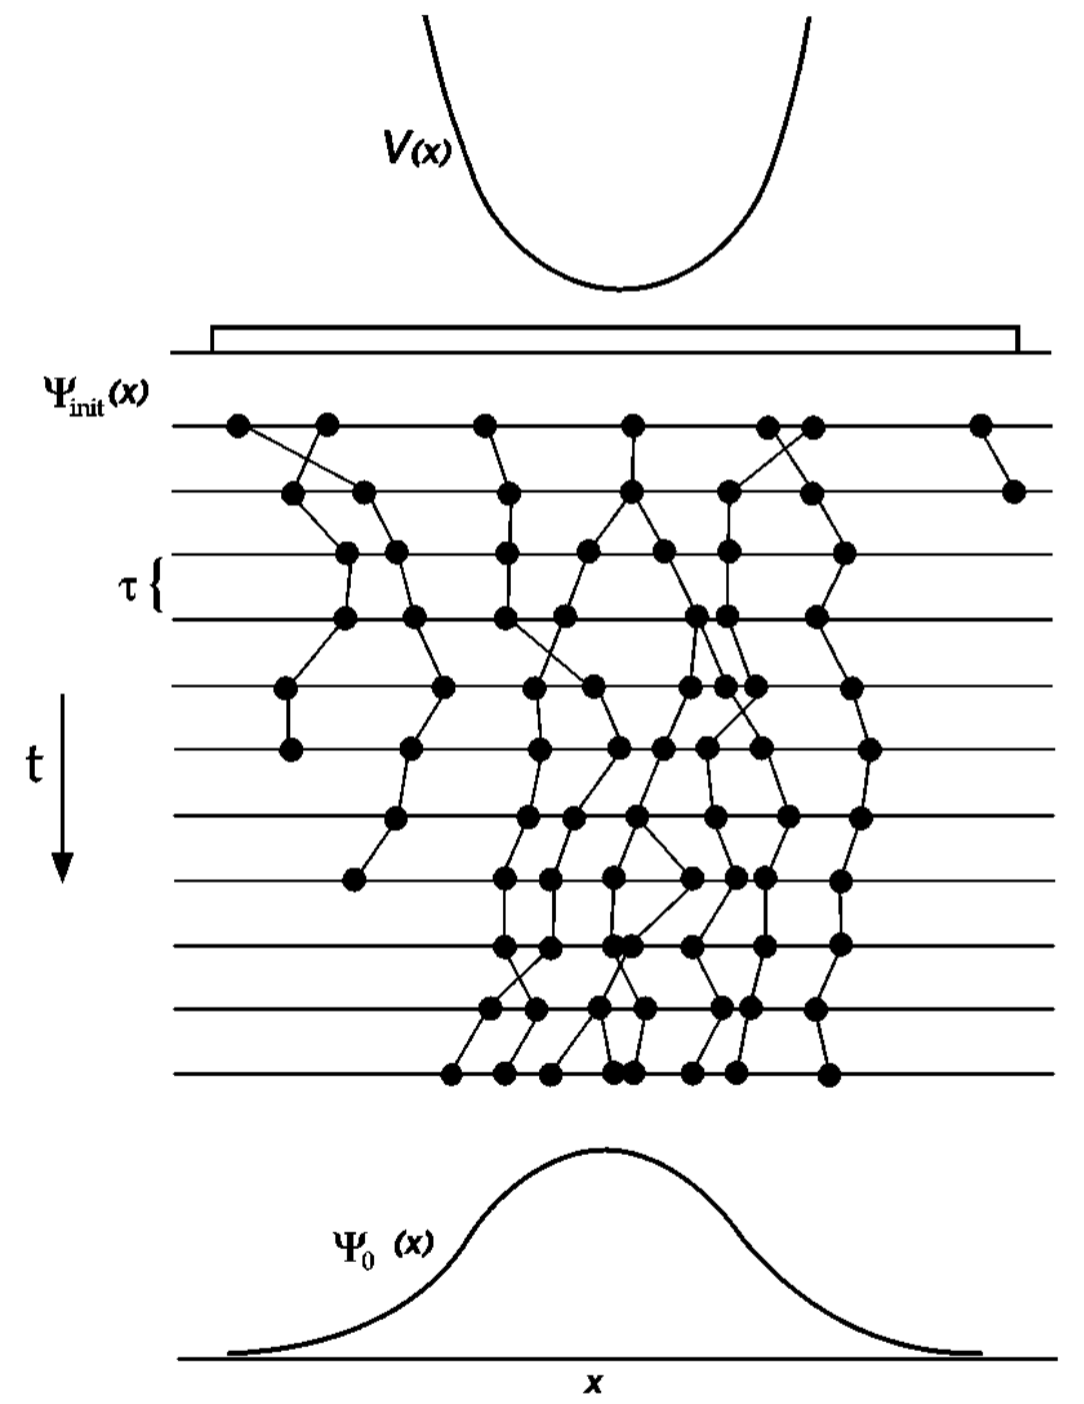
\includegraphics[width=0.4\textwidth]{figures/branching.png}
   \caption{Diagram describing the branching algorithm for Diffusion Monte Carlo (DMC). In this 1D example a particle is confined by the potential $V(x)$ and the trial wave function $\Psi_\text{init}(x)$ is propagated until it converges to the ground state wave function $\Psi_0(x)$. This diagram is from \cite{foulkes2001}.}
   \label{fig:branching}
\end{figure}

This sampling can have large uncertainties due to possible divergences in the branching weight in equation~\ref{equ:branchweight} as a result of particles getting too close or even coinciding. With the use of an importance function, $\Psi_I(\R)$ these fluctuations can be controlled without effecting the energy result. The importance function is used to bias the walker distributions toward $f(\R,t) = \Psi_T(\R,t)\Psi_I(\R)$ instead of $\Psi_T(\R,t)$ which effectively keeps the walkers away from locations where $\left|\Psi_T(\R,t)\right|^2$ is small.

This can be seen by multiplying Equation~\ref{equ:diffusion} by $\Psi_I(\R)$ and rewriting it in terms of $f(\R)$ as
\begin{equation}
   -\frac{1}{2}\nabla^2 f(\R,t) + \nabla\cdot\left[\mathbf{v}_D(\R) f(\R,t)\right] + \left[E_L(\R)-E_0\right]f(\R,t) = -\frac{\partial}{\partial t} f(\R,t),
\end{equation}
where $\mathbf{v}_D(R)$ is the drift velocity, defined as
\begin{equation}
   \mathbf{v}_D(\R) = \Psi_I(\R)^{-1}\nabla\Psi_I(\R) = \nabla \text{ln}\left|\Psi_I(\R)\right|.
\end{equation}
The drift velocity is responsible for pushing walkers away from areas of low $\left|\Psi_T(\R,t)\right|^2$. In practice the importance function is accounted for by directly sampling from
\begin{equation}
   G(\R',\R,\Delta\tau)\frac{\braket{\R}{\Psi_I}}{\braket{\R'}{\Psi_I}}
\end{equation}
instead of from the Green's function.

It is difficult to operate through the Green's function and so often observables are computed via mixed expectation values.
\begin{equation}
   \left<\mathcal{O(\tau)}\right>\text{mixed} = \frac{\bra{\Psi(\tau)}\mathcal{O}\ket{\Psi_T}}{\braket{\Psi(\tau)}{\Psi_T}}
\end{equation}
The true operator expectation value can approximately be written in terms of mixed expectation values \cite{pudliner1997} as
\begin{equation}
   \left<\mathcal{O(\tau)}\right> \approx 2\left<\mathcal{O(\tau)}\right>_\text{mixed} - \left<\mathcal{O}\right>_T,
   \label{equ:mixedexp}
\end{equation}
where
\begin{equation}
   \left<\mathcal{O}\right>_T = \frac{\bra{\Psi_T}\mathcal{O}\ket{\Psi_T}}{\braket{\Psi_T}{\Psi_T}}
\end{equation}
is the variational expectation value. Equation~\ref{equ:mixedexp} comes from a linear extrapolation of the mixed expectation value. For the Hamiltonian and operators that commute with the Hamiltonian the mixed expectation value is exactly the true expectation value for large time step. This can be seen directly with the Hamiltonian by splitting the Green's function up, to be used on either side of the Hamiltonian.
\begin{equation}
   \lim\limits_{\tau\rightarrow\infty}\left<H\right>_\text{mixed} = \frac{\bra{\Psi_T}e^{-H\tau/2}He^{-H\tau/2}\ket{\Psi_T}}{\bra{\Psi_T}e^{-H\tau/2}e^{-H\tau/2}\ket{\Psi_T}} = E_0
\end{equation}

The nuclear wave function is antisymmetric and will change sign as particle interact and exchange. As a result the oscillatory nature of the wave function requires positive and negative terms to cancel in the integral. Very accurate calculations must be done to accurately calculate these cancellations, and as a result very large uncertainties can be obtained. One approximate solution to this is the fixed-node approximation \cite{moskowitz1982}. The basic idea is that the trial wave function defines a nodal surface that is zero at the surface and changes sign across the surface. The wave functions are not allowed to cross the nodal surface. This maintains the upper bound principle of VMC, and is exact if the trial wave function, from which the nodal surface is defined, is exactly the ground state. This method assumes that the wave function is real, which is usually not the case with spin-isospin interactions. A generalization called the constrained path method works for real and complex wave functions alike \cite{wiringa2000}. The general idea is that walker configurations that have negative or zero overlap with the propagated wave function are discarded. This is only an approximate approach that depends on the choice of $\Psi_T(\R)$ and does not guarantee an upper bound on the energy. To this day there is active research looking for efficient ways to solve the Fermi-sign problem in many-body quantum systems. In practice we follow the method used in \cite{zhang2003} by using the real part of the trial wave function as the importance function and setting the weight to zero for any configuration whose overlap with the propagated wave function is zero or negative. This guarantees that the weights will be real and positive.

The constraint gives a non-exact result, however better convergence to the exact answer can be obtained by generating a set of good configurations with the constraint and then releasing the constraint for typically 20 to 40 steps to calculate the energy. Small systems, $A\le4$, will often converge before the statistical error overwhelms the signal. For larger systems an exponential extrapolation is typically used to determine the final energy as in \cite{pudliner1997}.

The DMC algorithm can generally be written as follows.
\begin{enumerate}
   \item Generate a set of random walkers. These are typically from the results of a VMC calculation, which has no constraint and provides an upper bound in the energy.
   \item For each walker propose a move, $\R' = \R + \mathbf{\chi}$, where $\mathbf{\chi}$ is a vector of random numbers from the shifted Gaussian $\exp\left(\frac{m}{2\hbar^2\Delta\tau}\left(\R'-\R+2\frac{\nabla\Psi_I(\R')}{\Psi_I(\R')}\right)^2\right)$.
   \item For each walker calculate the weight $w(\R')=\exp\left(-\left(\frac{E_L(\R')+E_L(\R)}{2}-E_0\right)\Delta\tau\right)$.
   \item Do branching.
   \item Calculate and collect the observables and uncertainties needed and increase the imaginary time by $\Delta\tau$.
   \item Repeat steps 2 through 5 until the uncertainties are small enough.
\end{enumerate}

The uncertainties are calculated by block averaging. The data we generate is inherently autocorrelated because each step in the Markov chain depends on the last. This will underestimate the statistical error in our calculation. The idea of block averaging is to form blocks in our data such that the average over each block is not correlated with the last block. This gives us a good estimate for the statistical uncertainty. In practice the block size is chosen so that the error estimate will not increase as the block size is increased. This is illustrated in the sample data shown in Figure~\ref{fig:blockaverage}.
\begin{figure}[h!]
   \centering
   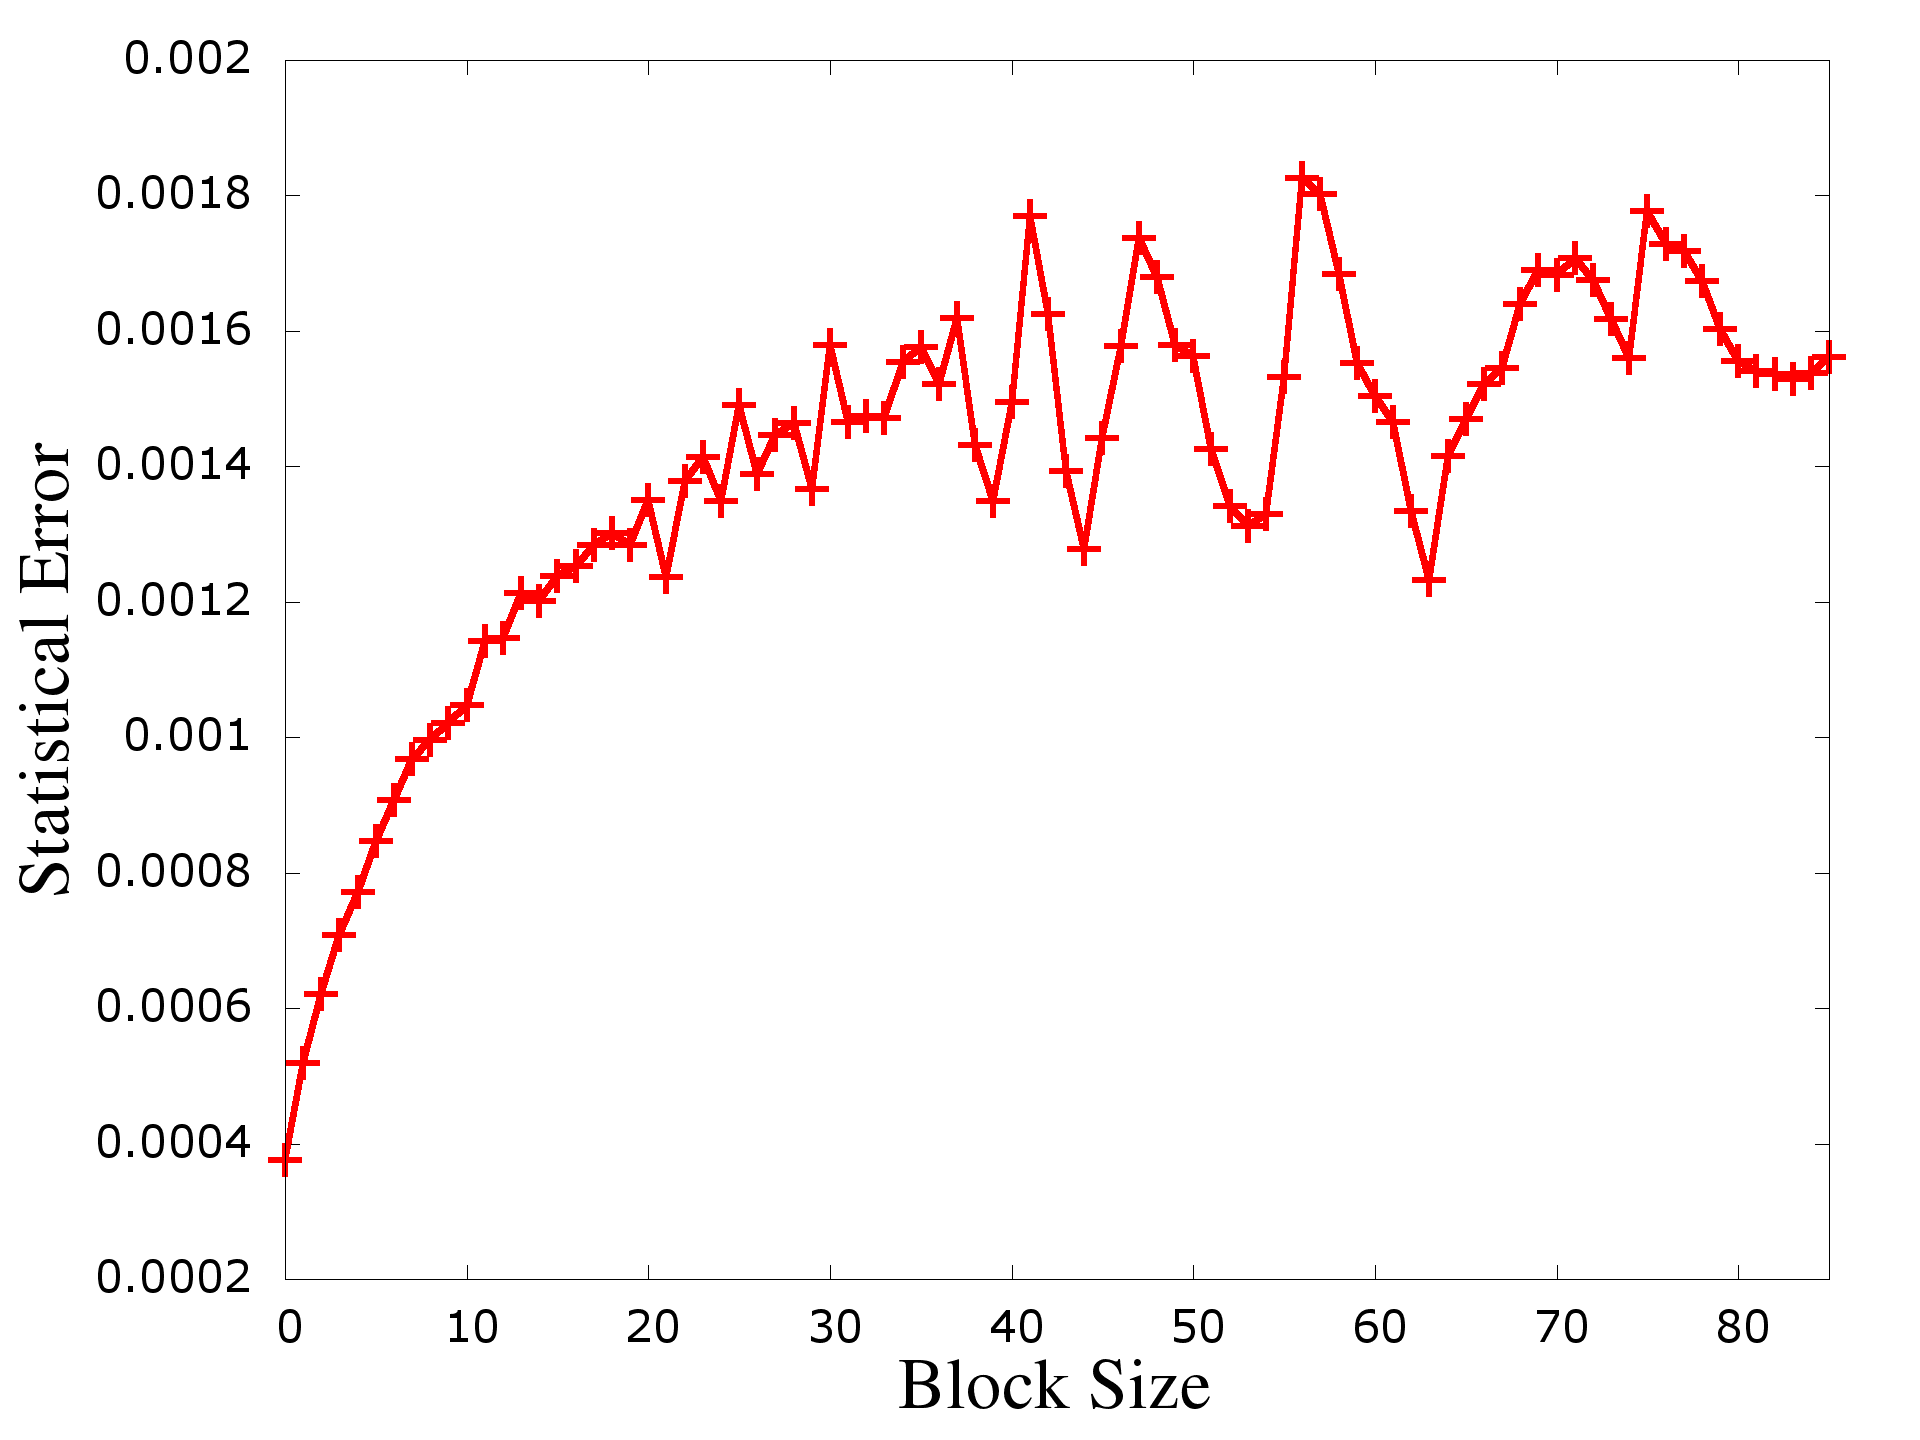
\includegraphics[width=0.7\textwidth]{figures/blockaverage.png}
   \caption{Sample data showing the convergence of the statistical uncertainty as the block size is increased. An appropriate block size for this data would be about 35, where the errors stop increasing with block size.}
   \label{fig:blockaverage}
\end{figure}

Good reviews of this method can be found in Refs. \cite{foulkes2001} and  \cite{carlson2015}. DMC only accounts for spin-isospin independent Hamiltonians, unlike Green's function Monte Carlo (GFMC) and auxiliary field diffusion Monte Carlo (AFDMC) which follow DMC for sampling spatial states but use two different methods to sample spin-isospin states. For each set of spatial integrals there is a sum over all of the spin and isospin states. GFMC evaluates this sum explicitly. This is inefficient as the number of spin states scales as
\begin{equation}
   \frac{A!}{Z!(A-Z)!}2^A
\end{equation}
where $A$ is the number of nucleons and $Z$ is the number of protons.
%The number of possible spin states given $A$ nucleons is $2^A$. The number of isospin states given $A$ nucleons and $Z$ protons can be reduced to ${A \choose Z}$ states leaving us with a total of $2^A {A \choose Z}$ spin-isospin states.
The number of states and the number of operators required for the trial wave function increase exponentially as the number of nucleons increases. To date, the largest nuclei that can be calculated with GFMC is ${}^{12}C$ \cite{lovato2013,lovato2014,lovato2015}. AFDMC was developed as an alternative to the explicit sum over spin-isospin states that GFMC performs.

\subsection{Auxiliary Field Diffusion Monte Carlo}
\label{sec:AFDMC}
To overcome the exponentially large number of spin-isospin states that have to be summed in GFMC, AFDMC was developed in 1999 \cite{schmidt1999} to sample spin and isospin states and, in analogy to moving the position of each walker, rotate the spin and isospin of each walker. The walkers are defined by the three spatial positions and amplitude for each particle to be in each of the four possible spin-isospin states $\ket{s} = \ket{p\uparrow,p\downarrow,n\uparrow,n\downarrow}$. The Hamiltonian can then be broken up into spin-isospin independent $H_{SI}$ and spin-isospin dependent $H_{SD}$ parts. The spin-isospin dependent part only comes from the potential and can be written as $V_{SD}$. The propagator can be broken up to have the old propagator used in DMC, which is independent of spin and isospin, and a spin-isospin dependent piece.
\begin{equation}
   G(\R'S',\R S,\tau)=\bra{\R'}e^{-(H-E_0)\tau}\ket{\R}G_{SD}(\R'S',\R S,\tau)
\end{equation}
where the spin-isospin dependent part of the propagator is
\begin{equation}
   G_{SD}(\R'S',\R S,\dt) = \bra {\R'S'}e^{-V_{SD}\dt} \ket{\R S}.
\end{equation}
The spin-isospin dependent part of the potential can be written as
\begin{equation}
   V_{SD} = \sum\limits_{p=2}^{M}\sum\limits_{i<j} \vpij\Opij,
\end{equation}
where M is the number of operators (e.g. $M=6$ for the AV6$'$ potential or $M=18$ for the Argonne AV18 two-body potential \cite{wiringa1984}). In this study I have used the standard AV6$'$ potential which includes the operators $\si\cdot\sj$, $\ti\cdot\tj$, $\si\cdot\sj \ti\cdot\tj$, $S_{ij}$ and $S_{ij} \ti\cdot\tj$, where $S_{ij} = 3\si\cdot\hat{r}_{ij}\sj\cdot\hat{r}_{ij}-\si\cdot\sj$. Here the $\mathbf{\si}$ and $\mathbf{\ti}$ operators are the Pauli matrices applied to spin and isospin of the $i$-th particle respectively.

AFDMC samples the spin and isospin states by expressing the operators in terms of squared single-particle particle operators which are transformed via the Hubbard-Stratanovich transformation. This can be done if the operators are expressed in the more convenient form
\begin{equation}
   V_{SD} = \frac{1}{2}\sum\limits_{i,\alpha,j,\beta} \sigma_{i,\alpha}A^{\sigma}_{i,\alpha,j,\beta}\sigma_{j,\beta}
      + \frac{1}{2}\sum\limits_{i,\alpha,j,\beta} \sigma_{i,\alpha}A^{\sigma\tau}_{i,\alpha,j,\beta}\sigma_{j,\beta}\ti\cdot\tj
      + \frac{1}{2}\sum\limits_{i,j} A^{\tau}_{i,j}\ti\cdot\tj,
   \label{equ:VwithA}
\end{equation}
where we have defined new $A$ matrices. The $A$ matrices are written in terms of the $\vpij$ functions above. For example the simplest matrix is the $A^{\tau}_{i,j}$ matrix which can be shown to be $A^{\tau}_{i,j} = v_{\tau}(r_{ij})$. There is a factor of one half in Eq.~\ref{equ:VwithA} because the sums go over all $i$ and $j$ particles instead of pairs for which $i<j$. These matrices are zero when $i=j$ and they are symmetric. We can also write these matrices in terms of their eigenvalues and eigenvectors.
\begin{align}
   &\sum\limits_{j,\beta} A^{\sigma}_{i,\alpha,j,\beta}\psi^{\sigma}_{n,j,\beta} = \lambda^{\sigma}_n\psi^{\sigma}_{n,i,\alpha} \\
   &\sum\limits_{j,\beta} A^{\sigma\tau}_{i,\alpha,j,\beta}\psi^{\sigma\tau}_{n,j,\beta} = \lambda^{\sigma\tau}_n\psi^{\sigma\tau}_{n,i,\alpha} \\
   &\sum\limits_{j} A^{\tau}_{i,j}\psi^{\tau}_{n,j} = \lambda^{\tau}_n\psi^{\tau}_{n,i}
\end{align}
Written in terms of these eigenvalues and eigenvectors the potential can be written as
\begin{equation}
   V_{SD} = \frac{1}{2}\sum\limits_{n=1}^{3A} \left(O_{n}^{\sigma}\right)^2 \lambda_n^{\sigma}
      + \frac{1}{2}\sum\limits_{\alpha=1}^{3}\sum\limits_{n=1}^{3A} \left(O_{n\alpha}^{\sigma\tau}\right)^2 \lambda_n^{\sigma\tau}
      + \frac{1}{2}\sum\limits_{\alpha=1}^{3}\sum\limits_{n=1}^{A} \left(O_{n\alpha}^{\tau}\right)^2 \lambda_n^{\tau},
\end{equation}
where the operators are given by
\begin{equation}
\begin{split}
   O_{n}^{\sigma} &= \sum\limits_{j,\beta} \sigma_{j,\beta}\psi_{n,j,\beta}^{\sigma} \\
   O_{n\alpha}^{\sigma\tau} &= \sum\limits_{j,\beta} \tau_{j,\alpha}\sigma_{j,\beta}\psi_{n,j,\beta}^{\sigma\tau} \\
   O_{n\alpha}^{\tau} &= \sum\limits_{j} \tau_{j,\alpha}\psi_{n,j}^{\tau}.
\end{split}
\end{equation}
These operators in the propagator now have the effect of rotating the spinors, analogous to diffusing the walkers in space. To reduce the order of the operators in the propagator from quadratic to linear we use the Hubbard-Stratanovich transformation.
\begin{equation}
   e^{-\frac{1}{2}\lambda O^2} = \frac{1}{\sqrt{2\pi}} \int dx e^{-\frac{x^2}{2} + \sqrt{-\lambda}x O}
\end{equation}
The variable $x$ is called an auxiliary field. Using the fact that there are $3A$ $O_{n}^{\sigma}$ operators, $9A$ $O_{n\alpha}^{\sigma\tau}$ operators and $3A$ $O_{n\alpha}^{\tau}$ operators, for a total of $15A$ operators, and by using the Hubbard-Stratanovich transformation we can write the spin-isospin dependent part of the propagator as
\begin{equation}
   G_{SD}(\R'S',\R S,\dt) = \bra{\R'S'}\prod\limits_{n=1}^{15A}\frac{1}{\sqrt{2\pi}}\int dx_n e^{-\frac{x_n^2}{2}}e^{\sqrt{-\lambda_n\dt} x_nO_n}\ket{\R S}.
   \label{equ:GSD}
\end{equation}
The spinors are rotated based on auxiliary fields sampled from the Gaussian with unit variance in Eq.~\ref{equ:GSD}. The sampling of the auxiliary fields is done in exactly the same way as the sampling of the spatial walkers in DMC, with the Markov chain Metropolis algorithm. Each sampled auxiliary field depends only on the previous sample and no more history than that.

Importance sampling can be included in the Auxiliary Field sampling in a similar way as described before with DMC. However, in practice it is done as follows. The $\Delta \R$ and $\Delta x_n$ are sampled by symmetric Gaussians and so the probability of $\Delta \R$ and $-\Delta \R$, and $\Delta x_n$ and $-\Delta x_n$ are the same. As a result the weight for the four possible combinations are sampled as
\begin{align}
   w_1 &= \frac{\braket{\Psi_I}{\R+\Delta \R, S'(x_n)}}{\braket{\Psi_I}{\R S}} e^{\left(-V_{SI}(\R+\Delta\R) - E_0\right)\dt} \\
   w_2 &= \frac{\braket{\Psi_I}{\R-\Delta \R, S'(x_n)}}{\braket{\Psi_I}{\R S}} e^{\left(-V_{SI}(\R-\Delta\R) - E_0\right)\dt} \\
   w_3 &= \frac{\braket{\Psi_I}{\R+\Delta \R, S'(-x_n)}}{\braket{\Psi_I}{\R S}} e^{\left(-V_{SI}(\R+\Delta\R) - E_0\right)\dt} \\
   w_4 &= \frac{\braket{\Psi_I}{\R-\Delta \R, S'(-x_n)}}{\braket{\Psi_I}{\R S}} e^{\left(-V_{SI}(\R-\Delta\R) - E_0\right)\dt},
\end{align}
and the sample with the largest weight is used. The weight for the chosen configuration, which is used for branching, is the average of the four weights
\begin{equation}
   W = \frac{1}{4}\sum\limits_{n=1}^4 w_n.
\end{equation}

\subsection{Hamiltonian}
One of the difficulties in many-body nuclear physics is finding an accurate Hamiltonian that is easy to calculate with the method you have selected. For QMC methods the Hamiltonian must be in configuration space and it must be local. Small degrees of non-locality can be addressed \cite{lynn2012,lynn2013}. Also, the nuclear physics Hamiltonian must be able to account for 2-body and 3-body interactions. The most generic form for the nuclear Hamiltonian then takes the form
\begin{equation}
   H = -\frac{\hbar^2}{2m}\sum\limits_i \nabla_i^2 + \sum\limits_{i<j} v_{ij} + \sum\limits_{i<j<k} V_{ijk} + \ldots.
\end{equation}
In principle there could be higher order terms included the in practice the two-nucleon NN interaction $v_{ij}$ and the three-nucleon interaction (TNI) $V_{ijk}$ are the only terms included as the importance of an $n$-nuclear potential decreases as $n$ increases. Calculations with only NN potentials will often underbind nuclei with $A>2$ and it has been shown that the inclusion of the TNI interaction improves this underbinding as well as level ordering in the excitation spectra of nuclei. This improvement has been shown in GFMC \cite{fantoni2008} as well as other methods such as the no-core shell model \cite{navratil2003}.

The NN potential takes the form
\begin{equation}
   v_{ij} = \sum\limits_{p=1}^M v_p(\r_{ij})\mathcal{O}^p_{ij},
\end{equation}
where $M$ is the number of operators begin used.
Two-nucleon potentials are often fit to NN scattering data and several very accurate models have been developed including the Nijmengen \cite{nagels1975,stoks1994}, CD-Bonn \cite{machleidt1996,machleidt2001}, and Argonne $v$18 (AV18) potentials \cite{wiringa1984,wiringa1995}. The Argonne potential is one of the most accurate and will be used in this work. The AV18 potential has 18 operators coming from one- and two-pion exchange as well as phenomenological sources. Often a subset of the AV18 potential is used, e.g. AV4$'$, AV6$'$, AV8$'$ or AV14$'$. These AV$n'$ potentials have kept only the top $n$ most important terms and are refit to scattering data at that level. A study of the successive importance of these terms up to $n=8$ compared with the full AV18 with and without three-nucleon potentials is given in \cite{wiringa2002}. The operators of the AV18 potential are
\begin{align}
   \mathcal{O}_{ij}^{p=1,8} &= \left[1,\si\cdot\sj,S_{ij},\mathbf{L}\cdot\mathbf{S}\right]\otimes\left[1,\ti\cdot\tj\right], \\
   \mathcal{O}_{ij}^{p=9,14} &= \left[\mathbf{L}^2,\mathbf{L}^2\si\cdot\sj,(\mathbf{L}\cdot\mathbf{S})^2\right]\otimes\left[1,\ti\cdot\tj\right], \\
   \mathcal{O}_{ij}^{p=15,18} &= \left[T_{ij},\si\cdot\sj T_{ij},S_{ij}T_{ij},\tau_i^2+\tau_j^2\right],
\end{align}
where the tensor term is $S_{ij} = 3\si\cdot\hat{r}_{ij}\sj\cdot\hat{r}_{ij}-\si\cdot\sj$, the $\mathbf{L}\cdot\mathbf{S}$ term is the spin-orbit term, and the $T_{ij} = 3\tau_i^2\tau_j^2-\ti\cdot\tj$ is the isotensor term.

In this work the AV6$'$ potential is used, which includes all of the same operators as AV8$'$ except for those including the spin-orbit terms, $\left[1,\si\cdot\sj,S_{ij}\right]\otimes\left[1,\ti\cdot\tj\right]$. The functions multiplying the AV6$'$ operators are shown in figure \ref{fig:vij}.
\begin{figure}[h!]
   \centering
   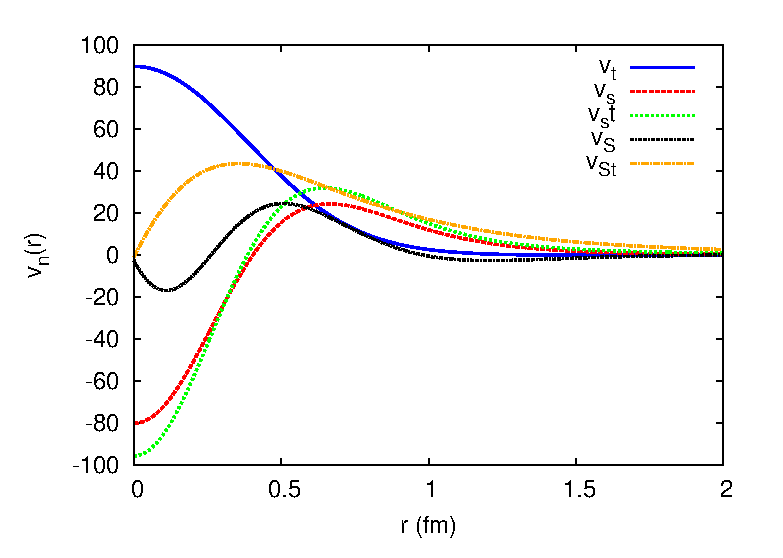
\includegraphics[width=0.7\textwidth]{figures/vij.eps}
   \caption{The functions multiplying the AV6$'$ operators as a function of nucleon separation. The central operator is excluded to show the spin-isospin terms with better detail. The $v_s$ represents the spin operators, $v_t$ the isospin operators, $v_{st}$ the spin-isospin operators, $v_S$ the tensor, and $v_{St}$ the tensor-isospin operators.}
   \label{fig:vij}
\end{figure}

The AV6$'$ can be broken up in Cartesian coordinates including 39 operators, 3 from $\tau$, 9 from $\sigma$, and 27 from $\sigma\tau$ terms. This can be done by writing the potential in the form
\begin{equation}
   \sum\limits_p v_p(\r_{ij})\mathcal{O}^p_{ij} = v_1(\r_{ij}) + \sum\limits_\alpha \t_{i\alpha}A^\tau_{ij}\t_{j\alpha} + \sum\limits_{\alpha,\beta} \s_{i\alpha}A^\sigma_{ij}\s_{j\beta} + \sum\limits_{\alpha,\beta,\gamma} \s_{i\alpha}\t_{i\gamma}A^{\sigma\tau}_{ij}\s_{j\beta}\t_{j\gamma},
\end{equation}
where the matrices are given by
\begin{align}
   A^\tau_{ij} &= v_2(\r_{ij}), \\
   A^\sigma_{ij} &= v_3(\r_{ij})\delta_{\alpha\beta} + v_5(\r_{ij})(3\rij^\alpha\rij^\beta-\delta_{\alpha\beta}), \\
   A^{\sigma\tau}_{ij} &= v_5(\r_{ij})\delta_{\alpha\beta} + v_6(\r_{ij})(3\rij^\alpha\rij^\beta-\delta_{\alpha\beta}).
\end{align}
This is a simple way to break up the AV6$'$ potential but a more efficient breakup can be used in which only 15 operators are needed. This is achieved by using $\rij$ as the first basis function and then using two additional orthogonal basis functions. This reduces the $\rij^\alpha\rij^\beta$ term in the matrices to $\delta_{\alpha\beta}$. This potential can then be written as
\begin{equation}
   \sum\limits_p v_p(\r_{ij})\mathcal{O}^p_{ij} = v_1(\r_{ij}) + \sum\limits_\alpha \t_{i\alpha}A^\tau_{ij}\t_{j\alpha} + \sum\limits_{\alpha} \s_{i\alpha}A^\sigma_{ij}\s_{j\alpha} + \sum\limits_{\alpha,\gamma} \s_{i\alpha}\t_{i\gamma}A^{\sigma\tau}_{ij}\s_{j\alpha}\t_{j\gamma},
\end{equation}
where the matrices are given by
\begin{align}
   A^\tau_{ij} &= v_2(\r_{ij}), \\
   A^\sigma_{ij} &= v_3(\r_{ij}) + 2v_5(\r_{ij}), \\
   A^{\sigma\tau}_{ij} &= v_5(\r_{ij}) + 2v_6(\r_{ij}),
\end{align}
where it is easy to see that there are 3 $\tau$, 3 $\sigma$, and 9 $\sigma\tau$ terms for a total of 15 operators in this basis.

Calculations with $A\le2$ are well described by the NN potentials, however for any system with $A\ge3$ the 3-nucleon force is needed to accurately describe the system. The phenomenological 3-nucleon forces that are typically employed in AFDMC calculations are the older Urbana and newer Illinois potentials. The Urbana IX (UIX) potential is built using the two-pion three-nucleon interaction, which can be written as
\begin{equation}
\begin{split}
   V_{2\pi3N} = \sum\limits_\text{cycl.} &A_{2\pi}\{\t_1\cdot\t_2,\t_1\cdot\t_3\} \{(S_{12}T(\r_{12})+\s_1\cdot\s_2 Y(\r_{12})),(S_{13}T(\r_{13})+\s_1\cdot\s_3 Y(\r_{13}))\} \\
      + &C_{2\pi}\left[\t_1\cdot\t_2,\t_1\cdot\t_3\right] \left[(S_{12}T(\r_{12})+\s_1\cdot\s_2 Y(\r_{12})),(S_{13}T(\r_{13})+\s_1\cdot\s_3 Y(\r_{13}))\right] \\
      + &B(\r_{12},\r_{13})\{\t_1\cdot\r_2,\t_1\cdot\t_3\}\{(S_{12}+\s_1\cdot\s_2),(S_{13}+\s_1\cdot\s_3)\},
\end{split}
\end{equation}
where the sum is a cyclic sum over 1, 2, and 3. The $\{~,~\}$ and $[~,~]$ are anticommutators and commutators and the $Y(r)$ and $Y(r)$ are the radial Yukawa and one-pion exchange interactions as described in \cite{carlson1983},
\begin{align}
   Y(r) &= \frac{e^{-\mu r}}{\mu r} Y_\text{cut}(r) \\
   T(r) &= \left(1+\frac{3}{\mu r} + \frac{3}{\mu^2 r^2}\right)\frac{e^{-\mu r}}{\mu r} T_\text{cut}(r),
\end{align}
where $Y_\text{cut}(r)$ and $T_\text{cut}(r)$ are the cutoff functions for the Yukawa and one-pion exchange terms respectively. The $B(\r_{12},\r_{13})$ term comes from $\pi$N s-wave scattering. The UIX potential is fit to the ground states of $^3$H and $^4$He. For details about the construction and results obtained with this potential I refer the reader to \cite{carlson1983, pudliner1996, pudliner1997}.

The Illinois-7 (IL7) potential \cite{pieper2001} contains two-pion three-nucleon interactions in both the s-wave and p-wave, as well as a three-pion exchange and three-nucleon contact interactions. The IL7 potential has been fit to the low-lying spectra of nuclei with $A=3$ to nuclei with $A=10$. These phenomenological potentials have been used to calculate many properties of light nuclei with high accuracy using both the GFMC and AFDMC methods.

Despite the accuracy of these potentials they have little direct connection to the underlying theory of QCD. In recent years a set of nuclear potentials has been developed from a chiral effective field theory ($\chi$EFT) framework that can be used with nuclear QMC methods such as GFMC and AFDMC \cite{epelbaum2009,machleidt2011}. These potentials are local up the next-to-next-to leading order (N$^2$LO) and so QMC calculations can use potentials up to this order. Good results using these potentials have been obtained with both GFMC \cite{lynn2014} and AFDMC \cite{lonardoni2018}.

All calculations here have been done with the AV6$'$ potential to reduce computation requirements as well as to better focus on the improvements made by improved wave functions. It would be straightforward to do any of these calculations with the three-nucleon and the $\chi$EFT potentials.


\section{Wave function with independent pair correlations}
One of the simplest many particle wave functions is a antisymmetrized product of single particle orbitals. This is often called a Slater Determinant. This wave function represents that long range part of the interactions leaving our short range correlations. The simplest short range correlation that can be formed is Jastrow-like correlation only dependent on space \red{Add reference here}.
\begin{equation}
   \ket{\psi_T} = \prod\limits_{i<j}f(r_{ij}) \ket{\phi}
\end{equation}
This does not include any spin-isospin correlations, and also is not cluster decomposable. The most general form for correlations that can be spin-isospin dependent and are cluster decomposable is an exponential form.
\begin{equation}
   \ket{\psi_T} = \prod\limits_{i<j}f_c(r_{ij}) e^{\sum\limits_p\fpij\Opij} \ket{\phi}
\end{equation}
If we then assume that the correlations are small we can then expand the exponential to first order getting
\begin{equation}
   \ket{\psi_T} = \prod\limits_{i<j}f_c(r_{ij}) \left(1+\sum\limits_p\fpij\Opij\right) \ket{\phi}.
\end{equation}
From here I'm going to expand this out showing why we previously have use the wave function that we did, and why we are adding the independent pair terms as we have. I will do this by assuming $A=3$ for convenience. Expanding this out we get
\begin{align}
   &\left[\f{c}{12}\left(1+\fO{p}{12}\right)\right]\left[\f{c}{13}\left(1+\fO{p}{13}\right)\right]\left[\f{c}{23}\left(1+\fO{p}{23}\right)\right] \\
   &=\f{c}{12}\f{c}{13}\f{c}{23}\left(1+\fO{p}{12}+\fO{p}{13}+\fO{p}{23}\right. \\
   &~~~~~+\left.\fO{p}{12}\fO{q}{13}+\fO{p}{12}\fO{q}{23}+\fO{p}{13}\fO{q}{23}\right) \\
   &= \left[\prod\limits_{i<j}\f{c}{ij}\right]\left[1+\fOpij+\fOpij\fOqkl + \ldots \right].
\end{align}
In the example with $A=3$ we only get up to quadratic terms, but you can imagine many more terms if you have more particles. With previous calculations we have approximated this by only taking up to the linear term.
\begin{equation}
   \ket{\psi_T} = \left[\prod\limits_{i<j}f_c(r_{ij})\right] \left[1+\fOpij\right] \ket{\phi}.
\end{equation}
What I have done here is kept some, but not all, of the quadratic terms.
\begin{equation}
   \ket{\psi_T} = \left[\prod\limits_{i<j}f_c(r_{ij})\right] \left[1+\fOpij\left(1 + \fOqklip\right)\right] \ket{\phi}
\end{equation}
The sum $\sum\limits_{\mathrm{k<l,ip}}$ is a sum over all of the $kl$ pairs that don't have a particle that matches either the $i^\mathrm{th}$ or the $j^\mathrm{th}$ particle. This is the independent pair sum.

\subsection{Fully Quadratic, and why there is a $\frac{1}{2}$}
It turns out that if you take all of the quadratic terms you get something like
\begin{equation}
   \ket{\psi_T} = \left[\prod\limits_{i<j}f_c(r_{ij})\right] \left[1+\fOpij + \frac{1}{2}\fOpij\sum\limits_{k<l,ij\ne kl}\sum\limits_q \fqkl\Oqkl\right] \ket{\phi}.
\end{equation}
You can see when when you work out the symmetrization operator (along with the sum over $i<j$ particle pairs. You have something like
\begin{equation}
   \mathcal{S} \prod\limits_{i<j} \left(1+\mathcal{O}_{ij}\right) = \frac{1}{A!}\sum\limits_{\{p\}}^{A!}\prod\limits_{i<j} \left(1+\mathcal{O}_{ij}\right),
\end{equation}
where $A!$ are the number of possible permutations for A particles. The product works out to look like
\begin{equation}
   (1+\mathcal{O}_{12})(1+\mathcal{O}_{13})\ldots(1+\mathcal{O}_{(A-1)(A)}).
\end{equation}
Since you never get the operators on the same particles before the permutations you will never get the same particles afterwards (so 1213 will never turn into 2525 or 2552 (which would be 2525)), and since operators on different particles commute you will always get sums like $i<j$. There will be $A!$ permutations and each permutation of the products will produce 1 of each of the sets of pairs. Each permutation will produce a 1246 for example, but they will be produced from different terms. The factor of a $\frac{1}{2}$ is simply because of the way I have written the sums. The way I've written the sums I get 1246 and 4612, but those are the same. If I was to write 
\begin{equation}
   \ket{\psi_T} = \left[\prod\limits_{i<j}f_c(r_{ij})\right] \left[1+\fOpij + \sum\limits_{ij<kl}\sum\limits_p \fpij\Opij \sum\limits_q \fqkl\Oqkl\right] \ket{\phi}.
\end{equation}
then the factor of a half goes away. \textit{The only problem is I've \textbf{ignored commutation terms} that come from switching 2412 to 1224 (wince the $f$ functions for the 2's don't commute)}. Notice that both quadratic wave functions scale as $A^4$ but with different factors. The number of 2-body terms in the fully quadratic scales as $\frac{1}{8}(A^4-2A^3-A^2+2A)$. You can figure this out by saying that there are $A(A-2)/2$ pairs, then there are $N(N-1)/2$ of those pairs, where $N$ is the number of pairs $N=A(A-1)/2$. The number of independent pair terms also scales as $A^4$, but as $\frac{1}{8}A(A-1)(A-2)(A-3)=\frac{1}{8}(A^4-6A^3+11A^2-6A)$.
\subsection{$f^p(r_{ij})$ functions in the correlations}
In the 2015 review they mention that the $f_{S,T}(r)$ functions are calculated from a Schr\"odinger-like equation
\begin{equation*}
   \left[-\frac{\hbar^2}{2\mu}\nabla^2+v_{S,T}(r)+\lambda_{S,T}(r)\right] = 0.
\end{equation*}
This equation comes from the fact that when two particles get close to eachother the potential get's really large, think Lennard-Jones potential that is infinite at 0. This gives large energies in the local energy unless something cancels it. The above equation is the result of trying to cancel these large potential terms. If particles 1 and 2 get close then $v(r_{ij})$ gets large and the corresponding derivative terms must cancel this. The dominant derivative term \red{I don't see where other terms would even come from} is the $\nabla^2$ term and the $\lambda$ encodes all the rest.


\section{Some notes about the Pfaffian wave function}
\red{Explain why it would be nice to have a pfaffian instead of a determinant and maybe mention some of the results related to superfluidity etc.}
Here are a few useful properties of the pfaffian of a skew-symmetric matrix.
\begin{enumerate}
   \item If you multiply row i and column i by a constant the resulting pfaffian will be multiplied by that constant. Just a row or column will multiply the pfaffian by the square root of that constant.
   \item Simultaneously interchanging two rows (and corresponding columns) will change the sign of the pfaffian.
   \item Adding the multiple of a row (and a corresponding addition with a column) to another row (and column) will not change the pfaffian.
\end{enumerate}

In the code there are a few things that I want to make sure I understand before I continue on.
\begin{enumerate}
   \item How they build the $\phi_{ij}$.
   \item How they calculate the pfaffian.
   \item How they calculate the potential
   \begin{enumerate}
      \item How do they do $\mathcal{O}_i\phi{ij}$, etc?
   \end{enumerate}
\end{enumerate}
To address how they build $\phi_{ij}$ let's start in wavebcs.f90 in the hpsi subroutine. The pf(2,2,A,A) parameter in the code I think would be best as pf(si,sj,i,j), where i and j are the particles and si and sj are the spins (up and down) of each neutron. The pf for 2 specific particles is passed to pairfn in orbital.f90, where it's calculated as
\begin{equation}
   pf(1,2)=vk(1)+\sum\limits_{i=2}^{nk} 2vk(i)\cos(\mathbf{k}_i\cdot\mathbf{r}),
\end{equation}
where the $vk$ are the amplitudes for each $k$ vector, and the factor of 2 accounts for the fact that each $i$ has a positive and a negative value, except for the zero case, $vk(1)$. For each set of particles the pf(2,1)=-pf(1,2) which is assume comes in when forming the singlet state. This is done when the radial part of the pair-state, pf is dotted with the spin states with dotsp in wavebcs.f90. It calculates for each particle i
\begin{align}
   dotsp(j) &= \ket{\uparrow}_i\ket{\uparrow}_j\phi(1,1)+\ket{\uparrow}_i\ket{\downarrow}_j\phi(1,2)+\ket{\downarrow}_i\ket{\uparrow}_j\phi(2,1)+\ket{\downarrow}_i\ket{\downarrow}_j\phi(2,2) \\
   &= \left(\ket{\uparrow}_i\ket{\downarrow}_j-\ket{\downarrow}_i\ket{\uparrow}_j\right)\phi(1,2) \\
   &= \text{spin-singlet * radial ij function},
\end{align}
where we have used $\phi(1,1)$ and $\phi(2,2)$ are zero and $\phi(1,2)=-\phi(2,1)$. Also, the $1$ and $2$ in $\phi$ refer to spin up and down respectively.

The $k$ vectors are stored in the code as $ak$ and are calculated, along with their weights in setupk in kshell.f90. It calculated $ak$ as $ak=2\pi/L*ik$ where $ik$ is the standard $k$ vectors (0,0,0), (0,0,1), etc, so the ak are ready to dot into the $\mathbf{r}$ vectors. The $vk$ are read into setupk.

The calculate the pfaffian the skew-symmetric matrix is first formed. In this case it's simply the dotsp calculated above for each particle i. In the code they also include single particle terms which are then used to build a determinant I believe. The pfaffian is then calculated using the subroutine pfaf from pfaffian.f90. \red{See Kevin's notes about how to calculate the pfaffian and decide how much to include in this, since it seems semi-complicated.}

\subsection{Calculate the Pfaffian}
First of all the pfaffian is defined as $\text{Pf}(A) = \mathcal{A}[\phi_{12}\phi_{34}\ldots\phi_{N-1,N}]$, where $A$ is the skew symmetrix matrix
\begin{equation}
   A = \begin{pmatrix} 
      0           &  \phi_{12}   &  \phi_{13}   &  \ldots   &  \phi_{1N} \\
      -\phi_{12}  &  0           &  \phi_{23}   &  \ldots   &  \phi_{2N} \\
      -\phi_{13}  &  -\phi_{23}  &  0           &  \ldots   &  \phi_{3N} \\
      \vdots      &  \vdots      &  \vdots      &  \ddots   &  \vdots    \\
      -\phi_{1N}  &  -\phi_{2N}  &  \phi_{3N}   &  \ldots   &  0         \\
\end{pmatrix}.
\end{equation}
To calculate the pfaffian the code uses the property that for block diagonal (each skew-symmetric) matricies the pfaffian can be written as
\begin{equation}
   \text{Pf}(A) = \text{Pf}\begin{pmatrix} 
      A_1   &  0 \\
      0     &  A_2
\end{pmatrix}
   = \text{Pf}(A_1)\text{Pf}(A_2).
\end{equation}
So if you can use Gaussian elemination to write the matrix $A_1$ as something like
\begin{equation}
   A_1 = \begin{pmatrix} 
      0           &  \phi_{12} \\
      -\phi_{12}  &  0
\end{pmatrix},
\end{equation}
and then Pf$(A)$ will be $\phi_{12}\text{Pf}(A_2)$. If the matrix is more than 4x4 then you could then use the process again to calculate the pfaffian of $A_2$.

Kevin showed this for a 4x4 matrix. He showed that you could write the Gaussian eliminated block matrix as

\begin{equation}
A'' = \left (
\begin{array}{cccc}
0 & a_{12} & 0 & 0 \\
-a_{12}& 0 & 0 & 0 \\
0& 0 & 0 &
 a_{34}+\frac{a_{14}a_{23}}{a_{12}}-\frac{a_{13}a_{24}} {a_{12}} \\
0& 0 &
 -a_{34}-\frac{a_{14}a_{23}}{a_{12}}+\frac{a_{13}a_{24}} {a_{12}}
 &0 \\
\end{array}
\right )  \,.
\end{equation}

He also points out that this operation can be calculated as
\begin{equation}
\label{trans}
A'' =
\left (
\begin{array}{cccc}
1 & 0 & 0 & 0\\
0 & 1 & 0 & 0\\
\frac{a_{23}}{a_{12}} &-\frac{a_{13}}{a_{12}}& 1 & 0\\
\frac{a_{24}}{a_{12}} & -\frac{a_{14}}{a_{12}}&0 & 1\\
\end{array}
\right )
\underbrace{
\left (
\begin{array}{cccc}
0 & a_{12} & a_{13} & a_{14} \\
-a_{12}& 0 & a_{23} & a_{24} \\
-a_{13}& -a_{23} & 0 & a_{34} \\
-a_{14}& -a_{24} & -a_{34} &0 \\
\end{array}
\right )
}_{A}
\left (
\begin{array}{cccc}
1 & 0 & \frac{a_{23}}{a_{12}} & \frac{a_{24}}{a_{12}}\\
0 & 1 & -\frac{a_{13}}{a_{12}} & -\frac{a_{14}}{a_{12}}\\
0 & 0 & 1 & 0\\
0 & 0 & 0 & 1\\
\end{array}
\right )  \,.
\end{equation}


\section{Derive Exponential Wave Function}
The most general form of the fully correlated wave function is the exponentially correlated wave function given by
\begin{equation}
   \ket{\Psi_T} = \left[\prod\limits_{i<j}f_c(r_{ij})\right] e^{\sum\limits_{i<j,p}f_p(r_{ij})\Oijp} \ket{\Phi}
\end{equation}
The exponential is to maintain cluster decomposition of the wave function. The Jastrow spin-isospin independent correlations are handeled independent of my piece of the code and so I will ignore them here which effectively leaves me with
\begin{equation}
   \ket{\Psi_T} = e^{\sum\limits_{i<j,p}f_p(r_{ij})\Oijp} \ket{\Phi},
\end{equation}
where the operators in the sum are the standard $v6'$ operators, $\si\cdot\sj$, $\ti\cdot\tj$, $\si\cdot\sj \ti\cdot\tj$, $S_{ij}$ and $S_{ij} \ti\cdot\tj$, where $S_{ij} = 3\si\cdot\hat{r}_{ij}\sj\cdot\hat{r}_{ij}-\si\cdot\sj$. In an effort to write this an a sum of squared single particle operators (to be used with the Hubbard Stratanovich transformation) these operators can be written in the form
\begin{equation}
   \exp\left(\sum\limits_{i<j,p}f_p(r_{ij})\Oijp\right) = \exp\left(\frac{1}{2}\sum\limits_{i\alpha,j\beta} \sigma_{i\alpha}A^{\sigma}_{i\alpha,j\beta}\sigma_{j\beta}
      + \frac{1}{2}\sum\limits_{i\alpha,j\beta} \sigma_{i\alpha}A^{\sigma\tau}_{i\alpha,j\beta}\sigma_{j\beta}\ti\cdot\tj
      + \frac{1}{2}\sum\limits_{i,j} A^{\tau}_{i,j}\ti\cdot\tj\right).
\end{equation}
These matricies are simply another way to write the $f^p(r_{ij})$ function. Writting the operators in this form is discussed in more detail in appendix~\ref{app:hsprep}. In the code (in psicalc.f90) these matricies are actually called ``ftau(npart,npart)", ``fsig(3,npart,3,npart)" and ``fsigtau(3,npart,3,npart)". These matricies are zero when $i=j$, symmetric and can be written in terms of their eigenvalues and vectors.
\begin{align}
   &\sum\limits_{j\beta} A^{\sigma}_{i\alpha,j\beta}\psi^{\sigma}_{n,j\beta} = \lambda^{\sigma}_n\psi^{\sigma}_{n,i\alpha} \\
   &\sum\limits_{j\beta} A^{\sigma\tau}_{i\alpha,j\beta}\psi^{\sigma\tau}_{n,j\beta} = \lambda^{\sigma\tau}_n\psi^{\sigma\tau}_{n,i\alpha} \\
   &\sum\limits_{j} A^{\tau}_{i,j}\psi^{\tau}_{n,j} = \lambda^{\tau}_n\psi^{\tau}_{n,i}
\end{align}
The operators can then be written as
\begin{equation}
   \exp\left(\sum\limits_{i<j,p}f_p(r_{ij})\Oijp\right) = \exp\left(\frac{1}{2}\sum\limits_{n=1}^{3A} \left(O_{n}^{\sigma}\right)^2 \lambda_n^{\sigma}
      + \frac{1}{2}\sum\limits_{\alpha=1}^{3}\sum\limits_{n=1}^{3A} \left(O_{n\alpha}^{\sigma\tau}\right)^2 \lambda_n^{\sigma\tau}
      + \frac{1}{2}\sum\limits_{\alpha=1}^{3}\sum\limits_{n=1}^{A} \left(O_{n\alpha}^{\tau}\right)^2 \lambda_n^{\tau}\right),
\end{equation}
where the operators are given by
\begin{equation}
\begin{split}
   O_{n}^{\sigma} &= \sum\limits_{j,\beta} \sigma_{j,\beta}\psi_{n,j,\beta}^{\sigma} \\
   O_{n\alpha}^{\sigma\tau} &= \sum\limits_{j,\beta} \tau_{j,\alpha}\sigma_{j,\beta}\psi_{n,j,\beta}^{\sigma\tau} \\
   O_{n\alpha}^{\tau} &= \sum\limits_{j} \tau_{j,\alpha}\psi_{n,j}^{\tau}.
\end{split}
\end{equation}
Now this is ready to use with the Hubbard Stratanovich transformation
\begin{equation}
   e^{-\frac{1}{2}\lambda O^2} = \frac{1}{\sqrt{2\pi}} \int dx e^{-\frac{x^2}{2} + \sqrt{-\lambda}x O}.
\end{equation}
Writting this set of correlation operators in a more compact way,
\begin{equation}
    \exp\left(\sum\limits_{i<j,p}f_p(r_{ij})\Oijp\right) = \exp\left(\frac{1}{2}\sum\limits_{n=1}^{15A} \left(O_{n}\right)^2 \lambda_n^{\sigma}\right)
\end{equation}
allows for the application of the HS transformation, after breaking it into $15A$ exponentials and ignoring the commutation terms.
\begin{equation}
   \exp\left(\frac{1}{2}\sum\limits_{n=1}^{15A} \left(O_{n}\right)^2 \lambda_n^{\sigma}\right) = \prod\limits_{n=1}^{15A} \frac{1}{\sqrt{2\pi}}\int dx_n e^{-x_n^2/2}e^{\sqrt{\lambda_n}x_nO_n}.
\end{equation}

The auxiliary fields can then be drawn from the gaussian distribution, $\exp\left(-x_n^2/2\right)$ and the correlations can be written as follows.
\begin{equation}
   \Psi_T(R,S) = \bra{RS}\prod\limits_{n=1}^{15A} \frac{1}{N} \sum\limits_{\{x_n\}}^N\frac{1}{\sqrt{2\pi}}e^{\sqrt{\lambda_n}x_nO_n}\ket{\Phi}.
\end{equation}

\subsection{Cluster Decomposability}
A physical multi-particle system has the property of cluster decomposability. This is that when two systems $A_1$ and $A_2$, are separated by large distances their composite wavefunction will asymptotically approach
\begin{equation}
   \ket{A_1 + A_2} \rightarrow \ket{A_1}\ket{A_2}.
   \label{eq:clusterdecomposition}
\end{equation}
The exponentially correlated trial wave function is cluster decomposable. If a system were split into two parts $A_1$ and $A_2$, any pair correlation with a particle in each system would have no contribution to the total wave function because any such correlation would be zero inside the exponential. This is not a property held by the linear or quadratically correlated wave functions.

For example, a system of four particles split into two subsystems and separated by a large distance where the two systems are $A_{12}$ containing particles 1 and 2, and $A_{34}$ containing particles 3 and 4. Any correlations that correlate particles in different subsystems will be zero. For the linear correlated wave function this will leave the correlationsof the form
\begin{equation}
   \bra{RS}\left[1+f_p(r_{12})\mathcal{O}^p_{12}+f_p(r_{34})\mathcal{O}^p_{34}\right]\ket{\Phi},
\end{equation}
where there is an implicit sum over $p$ operators. This is not of the form $\ket{A_{12} + A_{34}} = \ket{A_{12}}\ket{A_{34}}$ and is thus not cluster decomposable. A similar analysis can be done for the quadratically correlated wave function.

One of the advantages to the exponentially correlated wave function is that is maintains cluster decomposibility. The most basic form for the exponentially correlated wave function ignoring spin-isospin independent Jastrow correlations is
\begin{equation}
   \Psi_T = \bra{RS} e^{\sum\limits_{i<j} f_p(r_{ij})\mathcal{O}^p_{ij}} \ket{\Phi}.
\end{equation}
Again, any correlations that correlate particles from the two different systems will be zero and the wave function becomes
\begin{align}
   \Psi_T &= \bra{RS} e^{f_p(r_{12})\mathcal{O}^p_{12} + f_p(r_{34})\mathcal{O}^p_{34}} \ket{\Phi} \\
   &= \bra{RS} e^{f_p(r_{12})\mathcal{O}^p_{12}} e^{f_p(r_{34})\mathcal{O}^p_{34}} \ket{\Phi}.
\end{align}
The walkers $\ket{RS}$ and states $\ket{Phi}$ can be broken up into parts that correspond to the different subsystems and so the wave function can be written as
\begin{equation}
   \Psi_T = {}_{12}\bra{RS}e^{f_p(r_{12})\mathcal{O}^p_{12}}\ket{\Phi}_{12} {}_{34}\bra{RS}e^{f_p(r_{34})\mathcal{O}^p_{34}}\ket{\Phi}_{34}.
\end{equation}
This is the same form as equation~\ref{eq:clusterdecomposition} and is thus a sully cluster decomposed wave function.

\section{Exponential of an Operator}
To start I'll write down the exponential correlations in their full form. They look something like this
\begin{equation}
   \prod\limits_{n=1}^{15A} \frac{1}{\sqrt{2\pi}}\int dx_n e^{-x_n^2/2}e^{\sqrt{-\lambda_n}x_nO_n}.
\end{equation}
This is after the Hubbard-Staratanovich transformation has been applied to the correlations so that the correlations can be sampled from single-particle operators. If they are sampled they take a form something like
\begin{equation}
   \prod\limits_{n=1}^{15A} \frac{1}{\sqrt{2\pi}}\sum\limits_{x_n}^N\frac{1}{N}e^{\sqrt{-\lambda_n}x_nO_n}.
\end{equation}
It might also be important to note that we have added plus-minus sampling to this\ldots but I'll add that and the square root of the matrix stuff in later.

Now I will talk about each individual operator that we have in the correlations. The 15A operators are $\tau_{\alpha i}$ (3A), $\sigma_{\alpha i}$ (3A), and $\sigma_{\alpha i}\tau_{\beta j}$ (9A). Assuming the basis is $\left|p\uparrow,p\downarrow,n\uparrow,n\downarrow\right>$ and stored as a column vector we can write the operators in matrix form as follows.
\begin{equation*}
\tau_x=
\begin{pmatrix}
    0 & 0 & 1 & 0 \\
    0 & 0 & 0 & 1 \\
    1 & 0 & 0 & 0 \\
    0 & 1 & 0 & 0
\end{pmatrix}
~~~~~~~\tau_y=
\begin{pmatrix}
    0 & 0 & -i & 0 \\
    0 & 0 & 0 & -i \\
    i & 0 & 0 & 0 \\
    0 & i & 0 & 0
\end{pmatrix}
~~~~~~~\tau_z=
\begin{pmatrix}
    1 & 0 & 0 & 0 \\
    0 & 1 & 0 & 0 \\
    0 & 0 & -1 & 0 \\
    0 & 0 & 0 & -1
\end{pmatrix}
\end{equation*}
\begin{equation*}
\sigma_x=
\begin{pmatrix}
    0 & 1 & 0 & 0 \\
    1 & 0 & 0 & 0 \\
    0 & 0 & 0 & 1 \\
    0 & 0 & 1 & 0
\end{pmatrix}
~~~~~~~\sigma_y=
\begin{pmatrix}
    0 & -i & 0 & 0 \\
    i & 0 & 0 & 0 \\
    0 & 0 & 0 & -i \\
    0 & 0 & i & 0
\end{pmatrix}
~~~~~~~\sigma_z=
\begin{pmatrix}
    1 & 0 & 0 & 0 \\
    0 & -1 & 0 & 0 \\
    0 & 0 & 1 & 0 \\
    0 & 0 & 0 & -1
\end{pmatrix}
\end{equation*}
\begin{equation*}
\sigma_x\tau_x=
\begin{pmatrix}
    0 & 0 & 0 & 1 \\
    0 & 0 & 1 & 0 \\
    0 & 1 & 0 & 0 \\
    1 & 0 & 0 & 0
\end{pmatrix}
~~~~~~~\sigma_x\tau_y=
\begin{pmatrix}
    0 & 0 & 0 & -i \\
    0 & 0 & -i & 0 \\
    0 & i & 0 & 0 \\
    i & 0 & 0 & 0
\end{pmatrix}
~~~~~~~\sigma_x\tau_z=
\begin{pmatrix}
    0 & 1 & 0 & 0 \\
    1 & 0 & 0 & 0 \\
    0 & 0 & 0 & -1 \\
    0 & 0 & -1 & 0
\end{pmatrix}
\end{equation*}
\begin{equation*}
\sigma_y\tau_x=
\begin{pmatrix}
    0 & 0 & 0 & -i \\
    0 & 0 & i & 0 \\
    0 & -i & 0 & 0 \\
    i & 0 & 0 & 0
\end{pmatrix}
~~~~~~~\sigma_y\tau_y=
\begin{pmatrix}
    0 & 0 & 0 & -1 \\
    0 & 0 & 1 & 0 \\
    0 & 1 & 0 & 0 \\
    -1 & 0 & 0 & 0
\end{pmatrix}
~~~~~~~\sigma_y\tau_z=
\begin{pmatrix}
    0 & -i & 0 & 0 \\
    i & 0 & 0 & 0 \\
    0 & 0 & 0 & i \\
    0 & 0 & -i & 0
\end{pmatrix}
\end{equation*}
\begin{equation*}
\sigma_z\tau_x=
\begin{pmatrix}
    0 & 0 & 1 & 0 \\
    0 & 0 & 0 & -1 \\
    1 & 0 & 0 & 0 \\
    0 & -1 & 0 & 0
\end{pmatrix}
~~~~~~~\sigma_z\tau_y=
\begin{pmatrix}
    0 & 0 & -i & 0 \\
    0 & 0 & 0 & i \\
    i & 0 & 0 & 0 \\
    0 & -i & 0 & 0
\end{pmatrix}
~~~~~~~\sigma_z\tau_z=
\begin{pmatrix}
    1 & 0 & 0 & 0 \\
    0 & -1 & 0 & 0 \\
    0 & 0 & -1 & 0 \\
    0 & 0 & 0 & 1
\end{pmatrix}
\end{equation*}

Now those are easy enough to figure out if you just look at the pauli matricies on a simple spin-1/2 system. But what we really want is the exponential of these matricies with an extra factor up top that looks something like
\begin{equation}
   e^{\sqrt{-\lambda_n}x_nO_n}.
\end{equation}
I'm going to rewrite this with an $i$ in it as
\begin{equation}
   e^{i\gamma O_n},
\end{equation}
where the $\gamma=\sqrt{\lambda_n}x_n$, for each particular operator. In this way the exponentiated matricies can be written in terms of regular matricies. Plugging this into Mathematica I get the following.
\footnotesize
\begin{equation*}
e^{i\gamma\tau_x}=
\begin{pmatrix}
    \cos\gamma & 0 & i\sin\gamma & 0 \\
    0 & \cos\gamma & 0 & i\sin\gamma \\
    i\sin\gamma & 0 & \cos\gamma & 0 \\
    0 & i\sin\gamma & 0 & \cos\gamma
\end{pmatrix}
e^{i\gamma\tau_y}=
\begin{pmatrix}
    \cos\gamma & 0 & \sin\gamma & 0 \\
    0 & \cos\gamma & 0 & \sin\gamma \\
    -\sin\gamma & 0 & \cos\gamma & 0 \\
    0 & -\sin\gamma & 0 & \cos\gamma
\end{pmatrix}
e^{i\gamma\tau_z}=
\begin{pmatrix}
    e^{i\gamma} & 0 & 0 & 0 \\
    0 & e^{i\gamma} & 0 & 0 \\
    0 & 0 & e^{-i\gamma} & 0 \\
    0 & 0 & 0 & e^{-i\gamma}
\end{pmatrix}
\end{equation*}
\begin{equation*}
e^{i\gamma\sigma_x}=
\begin{pmatrix}
    \cos\gamma & i\sin\gamma & 0 & 0 \\
    i\sin\gamma & \cos\gamma & 0 & 0 \\
    0 & 0 & \cos\gamma & i\sin\gamma \\
    0 & 0 & i\sin\gamma & \cos\gamma
\end{pmatrix}
e^{i\gamma\sigma_y}=
\begin{pmatrix}
    \cos\gamma & \sin\gamma & 0 & 0 \\
    -\sin\gamma & \cos\gamma & 0 & 0 \\
    0 & 0 & \cos\gamma & \sin\gamma \\
    0 & 0 & -\sin\gamma & \cos\gamma
\end{pmatrix}
e^{i\gamma\sigma_z}=
\begin{pmatrix}
    e^{i\gamma} & 0 & 0 & 0 \\
    0 & e^{-i\gamma} & 0 & 0 \\
    0 & 0 & e^{i\gamma} & 0 \\
    0 & 0 & 0 & e^{-i\gamma}
\end{pmatrix}
\end{equation*}
\scriptsize
\begin{equation*}
e^{i\gamma\sigma_x\tau_x}=
\begin{pmatrix}
    \cos\gamma & 0 & 0 & i\sin\gamma \\
    0 & \cos\gamma & i\sin\gamma & 0 \\
    0 & i\sin\gamma & \cos\gamma & 0 \\
    i\sin\gamma & 0 & 0 & \cos\gamma
\end{pmatrix}
e^{i\gamma\sigma_x\tau_y}=
\begin{pmatrix}
    \cos\gamma & 0 & 0 & \sin\gamma \\
    0 & \cos\gamma & \sin\gamma & 0 \\
    0 & -\sin\gamma & \cos\gamma & 0 \\
    -\sin\gamma & 0 & 0 & \cos\gamma
\end{pmatrix}
e^{i\gamma\sigma_x\tau_z}=
\begin{pmatrix}
    \cos\gamma & i\sin\gamma & 0 & 0 \\
    i\sin\gamma & \cos\gamma & 0 & 0 \\
    0 & 0 & \cos\gamma & -i\sin\gamma \\
    0 & 0 & -i\sin\gamma & \cos\gamma
\end{pmatrix}
\end{equation*}
\begin{equation*}
e^{i\gamma\sigma_y\tau_x}=
\begin{pmatrix}
    \cos\gamma & 0 & 0 & \sin\gamma \\
    0 & \cos\gamma & -\sin\gamma & 0 \\
    0 & \sin\gamma & \cos\gamma & 0 \\
    -\sin\gamma & 0 & 0 & \cos\gamma
\end{pmatrix}
e^{i\gamma\sigma_y\tau_y}=
\begin{pmatrix}
    \cos\gamma & 0 & 0 & -i\sin\gamma \\
    0 & \cos\gamma & i\sin\gamma & 0 \\
    0 & i\sin\gamma & \cos\gamma & 0 \\
    -i\sin\gamma & 0 & 0 & \cos\gamma
\end{pmatrix}
e^{i\gamma\sigma_y\tau_z}=
\begin{pmatrix}
    \cos\gamma & \sin\gamma & 0 & 0 \\
    -\sin\gamma & \cos\gamma & 0 & 0 \\
    0 & 0 & \cos\gamma & -\sin\gamma \\
    0 & 0 & \sin\gamma & \cos\gamma
\end{pmatrix}
\end{equation*}
\begin{equation*}
e^{i\gamma\sigma_z\tau_x}=
\begin{pmatrix}
    \cos\gamma & 0 & i\sin\gamma & 0 \\
    0 & \cos\gamma & 0 & -i\sin\gamma \\
    i\sin\gamma & 0 & \cos\gamma & 0 \\
    0 & -i\sin\gamma & 0 & \cos\gamma
\end{pmatrix}
e^{i\gamma\sigma_z\tau_y}=
\begin{pmatrix}
    \cos\gamma & 0 & \sin\gamma & 0 \\
    0 & \cos\gamma & 0 & -\sin\gamma \\
    -\sin\gamma & 0 & \cos\gamma & 0 \\
    0 & \sin\gamma & 0 & \cos\gamma
\end{pmatrix}
e^{i\gamma\sigma_z\tau_z}=
\begin{pmatrix}
    e^{i\gamma} & 0 & 0 & 0 \\
    0 & e^{-i\gamma} & 0 & 0 \\
    0 & 0 & e^{-i\gamma} & 0 \\
    0 & 0 & 0 & e^{i\gamma}
\end{pmatrix}
\end{equation*}
\normalsize

\section{Write potential as squared ops for AFDMC}
\label{app:hsprep}
The spin-isospin dependent potential can be written in the form
\begin{equation}
   V = \sum\limits_p\sum\limits_{i<j} u^p(\rij)\Oijp.
\end{equation}
I'm going to just write this out in terms of the simplest set of terms, the $\ti\cdot\tj$ terms.
\begin{align}
   V &= \sum\limits_{i<j} u^\tau(\rij)\Oijp \\
   &= \sum\limits_{i<j} u^\tau(\rij)\left(\tau_{ix}\tau_{jx}+\tau_{iy}\tau_{jy}+\tau_{iz}\tau_{jz}\right) \\
   &= \sum\limits_{i<j} u^\tau(\rij)\ti\cdot\tj \\
   &= \sum\limits_\alpha\sum\limits_{i<j} u^\tau(\rij)\tia\tja.
\end{align}
These can be rewritten in terms in a martix made of of the $u$ values. In the case of the $\tau$ operators this is simple because $\Aijt=u^\tau(\rij)$. If I rewrite the potential using this, and doing a full sum over all i and j and then dividing by 2 I get
\begin{equation}
   V = \frac{1}{2}\sum\limits_{\alpha,i,j} \Aijt\tia\tja
\end{equation}
Now I want to write this matrix in terms of it's eigenvalues and eigenvectors, which are defined as
\begin{equation}
   A^{\tau}\psi_n^\tau=\lambda_n^\tau\psi_n^\tau,
\end{equation}
or if you want to write them in the matrix multiplication form
\begin{equation}
   \sum\limits_j\Aijt\psi_{n,j}^\tau = \lambda_n^\tau\psi_{n,i}^\tau.
\end{equation}
Now I want to write out the $A$ matrix in terms of it's eigenvalues and eigenvectors. I do this using eigenvector decompositon. This is defined as
\begin{equation}
   A=Q\Lambda Q^{-1},
\end{equation}
where $Q$ is the matrix of eigenvectors (so $Q_{ab}=\psi_{ab}$, the $a^{th}$ eigenvector for the $b^{th}$ particle, for example), and $\Lambda$ is the diagonal matrix of eigenvalues (so $\Lambda_{ab}=\delta_{ab}\lambda_a$). I didn't prove this, but it's roughly believable when you consider the eigenvalue equation, and doing it for each component. Also, if $Q$ is a symmetric square matrix, which it is for us, then you can write $Q^{-1}=Q^T$i. What we have in the potential is $\Aijt$, so we need to write the eigenvector decomposition in terms of the $ij^{th}$ entry. This can be done by using the definitions of matrix multiplication.
\begin{equation}
   (A\psi)_i = \sum\limits_jA_{ij}\psi_j
\end{equation}
\begin{equation}
   (AB)_{ij}=\sum\limits_\alpha A_{i\alpha} B_{\alpha j}
\end{equation}
I'll now use these two equations to get $A_{ij}$ from the definition of eigenvalue decomposition.
\begin{align}
   A_{ij} &= \left(Q\Lambda Q^T\right)_{ij} \\
   &=\sum\limits_\alpha\sum\limits_\beta Q_{i\beta}\Lambda_{\beta\alpha}Q^T_{\alpha j} \\
   &=\sum\limits_\alpha\sum\limits_\beta Q_{i\beta}\delta_{\beta\alpha}\lambda_\alpha Q^T_{\alpha j} \\
   &=\sum\limits_\alpha \lambda_\alpha Q_{i\alpha}Q^T_{\alpha j} \\
   &=\sum\limits_\alpha \lambda_\alpha \psi_{i\alpha}\psi_{j\alpha}
\end{align}
Now plug this into the equation that we had earlier for the potential to get
\begin{align}
   V &= \frac{1}{2}\sum\limits_{\alpha,i,j} \Aijt\tia\tja \\
   &= \frac{1}{2}\sum\limits_{\alpha,i,j}\sum\limits_n\lambda_n^\tau\psi_{i,n}\psi_{j,n}\tia\tja \\
   &= \frac{1}{2}\sum\limits_\alpha\sum\limits_n\left(\Ot\right)^2\lambda^\tau_n,
   \label{equ:Vtau}
\end{align}
where
\begin{equation}
   \Ot = \sum\limits_i \tau_{i\alpha}\psi^\tau_n.
\end{equation}
A similar analysis can be done for the $\Os$ and $\Ost$ operators.

\subsection{Importance Sampling}
\red{Fill in here!}

\subsection{Controlling the run away kinetic energy}


\section{One Pion Exchange potential}
\red{When I get a little for QFT under my belt I'll tackle this.}


\section{Alessandro Roggero's Correlations}
A possible form for spin iso-spin dependent correlations (tensor-tau only here) could be written as
\begin{equation}
   S_{ki} \rightarrow S'_{ki} = \left[1+\sum\limits_d^3\sum\limits_j^A f_{t\tau}(r_{ji})\hat{r}_{ji}\cdot\mathbf{\sigma}_i\tau_i^d\right]S_{ki},
\end{equation}
where the $S_{ki}$ is the usual Slater matrix, and the wave function is given by
\begin{equation}
   \Psi_T = \sum\limits_{y_d=\pm1} det[S'],
\end{equation}
there being a 6 total auxiliary fields ($\pm1$ for each of the three $y_d$). One of the main motivations for these correlations (I think) is their improvement on the 2-particle only coupling of the linear correlations, which still being relatively resonable to evaluate. Notice that when taking the determinant for an $A$ nucleon system there will be terms that couple from 1 to $A$ nucleons.

One of the issues with this wave function are the off diagonal correlations that are induced in the correlations function. For example with the 

\red{Add a little bit about Alessandro's correlations here}
One of the problems with the Alessandro's correlations is that they break $T^2$ and $T_z$ symmetry. That is, there are terms like \red{explain here how it breaks $T^2$ and $T_z$ and explain how linear or other correlations don't. Also explain how $J^2$ and $J_z$ are only broken if you include the $\sigma_i\cdot\sigma_j$ terms, which aren't included for now.}

One solution to this is to multiply the correlations by a term $e^{-\alpha T^2}$ such that alpha is large enough to exponentially reduce the $T^2$ and $T_z$ breaking. This added piece to the correlations would take the form
\begin{equation}
   \exp{\left(-\alpha T^2\right)} = \exp{\left(-\alpha \sum\limits_\beta \sum\limits_{i,j} \tau_{i\beta}\tau_{j\beta}\right)}.
\end{equation}
The Hubbard-Stratanovich transformation can be used on these operators by writting them as an exponential of squared one-body operators.
\begin{equation}
   \exp{\left(-\alpha T^2\right)} = \exp{\left(-\alpha \sum\limits_\beta \left(\sum\limits_{j} \tau_{j\beta}\right)^2\right)}.
\end{equation}
In a standard AFDMC calculation the sum over $\beta$ would then be approximated by a product over $\beta$ where the commutator terms are small as long as the factor $\alpha$ is small. However, $\alpha$ must be large in order to eliminate $T^2$ breaking terms from the wave function and thus this approximation can't be used. Instead we have used the identity
\begin{equation}
   \exp{\left(\sum\limits_\beta A_\beta\right)} = \mathcal{S}\prod\limits_\beta \exp(A_\beta),
\end{equation}
where the symmetrization operator $\mathcal{S}=\frac{1}{N!}\sum\limits_\pi P_\pi$, permutes the cartesian coordinates $\beta=xyz$. With this identity and the Hubbard-Stratanovich transformation we can write the correlations as
\begin{align}
   \exp{\left(-\alpha \sum\limits_\beta \left(\sum\limits_{j} \tau_{j\beta}\right)^2\right)}  &= \mathcal{S} \prod\limits_\beta \exp{\left(-\alpha \left(\sum\limits_{j} \tau_{j\beta}\right)^2\right)} \\
   &= \mathcal{S} \prod\limits_\beta \int dx_\beta \exp{\left(-x_\beta^2/2\right)}\exp{\left(i\sqrt{2\alpha}x_\beta \sum\limits_{j} \tau_{j\beta}\right)} \\
   &\approx \mathcal{S} \prod\limits_\beta \frac{1}{N}\sum\limits_{n=1}^N \exp{\left(i\sqrt{2\alpha}x_{n\beta} \sum\limits_{j} \tau_{j\beta}\right)},
\end{align}
where the sum over $n$ is a sum over the $N$ sampled configurations of the 3 auxiliary fields. The sum over $i$ can be brought out of the exponential as a product because the operators on different particles all commute. Also the symmetrization operator can be written as a sum over the $3!=6$ permutations of the $\beta$ coordinates giving us
\begin{equation}
   \frac{1}{6N} \prod\limits_j \sum\limits_{P(xyz)} \sum\limits_{n=1}^N \exp{\left(i\sqrt{2\alpha}x_{nx} \tau_{jx}\right)} \exp{\left(i\sqrt{2\alpha}x_{ny} \tau_{jy}\right)} \exp{\left(i\sqrt{2\alpha}x_{nz} \tau_{jz}\right)}
\end{equation}
The exponential operators on each particle look identical and can be written in a matrix representation as
\begin{align}
\exp\left(i\sqrt{2\alpha}x_{nx}\tau_{jx}\right) &=
\begin{pmatrix}
    \cos(a_{xn}) & 0 & i\sin(a_{xn}) & 0 \\
    0 & \cos(a_{xn}) & 0 & i\sin(a_{xn}) \\
    i\sin(a_{xn}) & 0 & \cos(a_{xn}) & 0 \\
    0 & i\sin(a_{xn}) & 0 & \cos(a_{xn}) \\
\end{pmatrix} \\
\exp\left(i\sqrt{2\alpha}x_{ny}\tau_{jy}\right) &=
\begin{pmatrix}
    \cos(a_{yn}) & 0 & \sin(a_{yn}) & 0 \\
    0 & \cos(a_y) & 0 & \sin(a_{yn}) \\
    -\sin(a_{yn}) & 0 & \cos(a_{yn}) & 0 \\
    0 & -\sin(a_{yn}) & 0 & \cos(a_{yn}) \\
\end{pmatrix} \\
\exp\left(i\sqrt{2\alpha}x_{nz}\tau_{jz}\right) &=
\begin{pmatrix}
    e^{ia_{zn}} & 0 & 0 & 0 \\
    0 & e^{ia_{zn}} & 0 & 0 \\
    0 & 0 & e^{-ia_{zn}} & 0 \\
    0 & 0 & 0 & e^{-ia_{zn}}
\end{pmatrix},
\end{align}
where $a_{xn}=\sqrt{2\alpha}x_{xn}$, $a_{yn}=\sqrt{2\alpha}x_{yn}$, $a_{zn}=\sqrt{2\alpha}x_{zn}$ and in our basis the iso-spin matricies are
\begin{equation}
\tau_x=
\begin{pmatrix}
    0 & 0 & 1 & 0 \\
    0 & 0 & 0 & 1 \\
    1 & 0 & 0 & 0 \\
    0 & 1 & 0 & 0
\end{pmatrix}
~~~~~~~\tau_y=
\begin{pmatrix}
    0 & 0 & -i & 0 \\
    0 & 0 & 0 & -i \\
    i & 0 & 0 & 0 \\
    0 & i & 0 & 0
\end{pmatrix}
~~~~~~~\tau_z=
\begin{pmatrix}
    1 & 0 & 0 & 0 \\
    0 & 1 & 0 & 0 \\
    0 & 0 & -1 & 0 \\
    0 & 0 & 0 & -1
\end{pmatrix}.
\end{equation}
Owing to the clean matrix representation of these operators the symmetrized product of exponential operators can be written as one matrix,
\begin{equation}
   \mathcal{M}_{jn} = \frac{1}{6} \sum\limits_{P(xyz)} =
\begin{pmatrix}
   A & 0 & B & 0 \\
   0 & A & 0 & B \\
   C & 0 & D & 0 \\
   0 & C & 0 & D
%    e^{ia_z}\cos(a_x)\sin(a_y) & 0 & \cos(a_z)\left(i\cos(a_y)\sin(a_x)+\cos(a_x)\sin(a_y)\right) & 0 \\
%    0 & e^{ia_z}\cos(a_x)\sin(a_y) & 0 & \cos(a_z)\left(i\cos(a_y)\sin(a_x)+\cos(a_x)\sin(a_y)\right) \\
%    \cos(a_z)\left(i\cos(a_y)\sin(a_x)-\cos(a_x)\sin(a_y)\right) & 0 & e^{-a_z}\cos(a_x)\cos(a_y) & 0 \\
%    0 & \cos(a_z)\left(i\cos(a_y)\sin(a_x)-\cos(a_x)\sin(a_y)\right) & 0 & e^{-a_z}\cos(a_x)\cos(a_y) \\
\end{pmatrix},
\end{equation}
where
\begin{align}
   A &= e^{ia_{zn}}\cos(a_{xn})\sin(a_{yn}) \\
   B &= \cos(a_{zn})\left(i\cos(a_{yn})\sin(a_{xn})+\cos(a_{xn})\sin(a_{yn})\right) \\
   C &= \cos(a_{zn})\left(i\cos(a_{yn})\sin(a_{xn})-\cos(a_{xn})\sin(a_{yn})\right) \\
   D &= e^{-a_{zn}}\cos(a_{xn})\cos(a_{yn}).
\end{align}
This matrix can then be build and operated on each of the particles.
\begin{equation} 
   \exp{\left(-\alpha T^2\right)} \approx \frac{1}{N} \prod\limits_{j=1}^A \sum\limits_{n=1}^N \mathcal{M}_{jn}
\end{equation}
\red{get rid of page break here}
\newpage

Equation 6 in Kevin's notes is
\begin{equation}
   P(J,M)\ket{\psi_T} = \frac{2J+1}{16\pi^2} \int_0^{4\pi} d\alpha \int_0^{\pi} d\beta \int_0^{2\pi} d\gamma \sin(\beta)D^{J*}_{M,M}(\alpha,\beta,\gamma)R(\alpha,\beta,\gamma)\ket{\psi_T}.
\end{equation}
For the isospin case where $T$=0 and $M$=0 this can be written as
\begin{equation}
   P(0,0)\ket{\psi_T} = \frac{1}{16\pi^2} \int_0^{4\pi} d\alpha \int_0^{\pi} d\beta \int_0^{2\pi} d\gamma \sin(\beta) e^{-i\sum\limits_i \tau_{zi}\alpha} e^{-i\sum\limits_i \tau_{yi}\beta} e^{-i\sum\limits_i \tau_{zi}\gamma} \ket{\psi_T},
\end{equation}
where $D^0_{0,0}(\alpha,\beta,\gamma)=1$ and the general rotation is $R(\alpha,\beta,\gamma)=e^{-\frac{i}{\hbar}T_z\alpha} e^{-\frac{i}{\hbar}T_y\beta} e^{-\frac{i}{\hbar}T_z\gamma}$, where $T_\delta = \hbar\sum\limits_i \tau_{\delta i}$.

Since the exponential of the pauli operators can be written easily as a matrix I have done this in the code.
\begin{equation}
   M_y(\beta)=ety=e^{-i\beta\tau_y} = \begin{pmatrix}
    \cos(\beta) & 0 & -\sin(\beta) & 0 \\
    0 & \cos(\beta) & 0 & -\sin(\beta) \\
    \sin(\beta) & 0 & \cos(\beta) & 0 \\
    0 & \sin(\beta) & 0 & \cos(\beta)
   \end{pmatrix}
\end{equation}
\begin{equation}
   M_z(\alpha)=etz=e^{-i\alpha\tau_z} = \begin{pmatrix}
   e^{-i\alpha} & 0 & 0 & 0 \\
   0 & e^{-i\alpha} & 0 & 0 \\
   0 & 0 & e^{i\alpha} & 0 \\
   0 & 0 & 0 & e^{i\alpha}
   \end{pmatrix}
\end{equation}
where the pauli matricies are
\begin{equation}
   ty= \begin{pmatrix}
   0 & 0 & -i & 0 \\
   0 & 0 & 0 & -i \\
   i & 0 & 0 & 0 \\
   0 & i & 0 & 0
   \end{pmatrix}, ~~~
   ty= \begin{pmatrix}
   1 & 0 & 0 & 0 \\
   0 & 1 & 0 & 0 \\
   0 & 0 & -1 & 0 \\
   0 & 0 & 0 & -1
   \end{pmatrix}.
\end{equation}
With these matricies defined this way the isospin projection can be written as
\begin{equation}
   P(0,0)\ket{\psi_T} = \frac{1}{16\pi^2} \int_0^{4\pi} d\alpha \int_0^{\pi} d\beta \int_0^{2\pi} d\gamma \sin(\beta) \prod_iM_z(\alpha,i) \prod_iM_y(\beta,i) \prod_iM_z(\gamma,i) \ket{\psi_T}.
\end{equation}


\newpage
\red{get rid of page break here}


\section{Results}
I have calculated binding energies with and without the independent pair correlations and compared the results. In both cases we have used the v6 potential and the same operators for the correlations. In each case the weights for each operator was determined variationally. Calculations were done for systems, $^4$He and $^{16}$O and the binding energies are reported in table \ref{tab:indpairresults} with and without independent pairs correlations and compared to the experimental value.

\begin{table}[h!]
   \centering
   \caption{Binding energies in MeV for $^4$He and $^{16}$O as calculated with and without independent pair correlations (IPC) compared to experimental energies.}
   \label{tab:indpairresults}
   \begin{tabular}{ccccc}
      \hline \hline
%       & Without IPC & With IPC & Expt.\\
       & Linear & IndPair & Quadratic & Expt.\\
      \hline
      $^4$He & -27.0(3) & -26.3(3) & -28.5(2) & -28.295\\
      $^{16}$O & -114(3) & -132(3) & -143.3(3) & -127.619\\
      \hline \hline
   \end{tabular}
\end{table}

I have also calculated the binding energy per nucleon of symmetric nuclear matter with density $\rho=0.16$fm$^{-1}$ of 28 particles with periodic boundary conditions. The energy per nucleon was -14.3(2) MeV without the independent pair correlations and -16.6(2) MeV with the independent pair correlations.

\begin{figure}[h!]
   \centering
   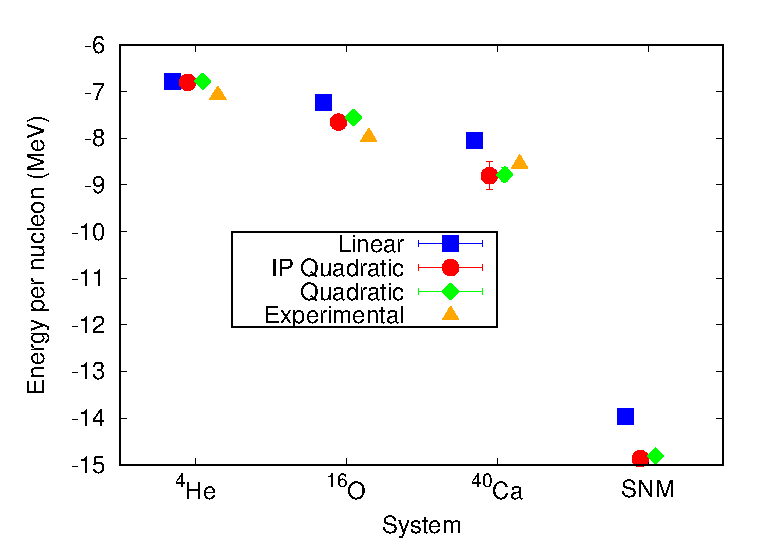
\includegraphics[width=0.5\textwidth]{energies.eps}
   \caption{Binding energies for ${}^4$He and ${}^{16}$O as calculated with linear, independent pair, and quadratic correlations. Also, the energy per nucleon of symmetric nuclear matter as calculated from 28 particles in a periodic box. All calculations are compared to their expected values.}
   \label{fig:energies}
\end{figure}


\bibliographystyle{abbrv}
\bibliography{references}

\end{document}
